\section{Non-axisymmmetric instability of artificial density bumps in
  layered discs}\label{density_bump} 
We first consider discs initialised with a density bump. Our aim here
is to examine the effect of (layered) viscosity on the RWI 
\emph{through the linear perturbation}. 
In general a density bump in a viscous disc will undergo viscous
spreading \citep{lyndenbell74}, but we can circumvent this 
by choosing the viscosity profile $\nu$ and initial cylindrical radial
velocity $v_{Ri}$ appropriately. 
Although artificial, this setup avoids 
the simultaneous evolution of the density bump subject to
axisymmetric viscous spreading and growth of
non-axisymmetric disturbances; only the latter of which is our focus. 


\subsection{Viscous equilibria for a radially structured
  disc}\label{visc_eq} 
%The RWI is a linear instability. That is, non-axisymmetric 
%disturbances grow exponentially with respect to a time-independent
%axisymmetric background. A convenient way to study the RWI is to
%initialize an inviscid disc with a density bump \citep[e.g.][]{li00}. 
%However, taking this approach with a viscous disc is problematic,
%because the density bump will generally undergoe viscous spreading 
%\citep{lyndenbell74}. 
 
In choosing $\rho_i$ and $\Omega_i$, we neglected radial
velocities and viscous forces in the steady-state vertical and
cylindrical radial momentum equations (Eq. \ref{vert_balance} and
Eq. \ref{init_vphi}, respectively). This is standard practice for
accretion disc modelling \citep[e.g.][]{takeuchi02}.   

However, $v_{R}$ and $\nu$ cannot be ignored in the azimuthal
momentum equation. Indeed, if a steady-state is desired, then the
conservation of angular momentum in a viscous disc implies special
relations between the viscosity, cylindrical radial velocity and
density field. %We do this for simulations in \S\ref{density_bump}.   


\subsubsection{Initial cylindrical radial velocity}
For axisymmetric flow with angular velocity that only depends on the
cylindrical radius, the azimuthal momentum equation reads 
\begin{align}\label{ang_mom_cons}
  R\rho v_R\frac{\p}{\p R}\left(R^2\Omega \right) = \frac{\p}{\p
    R}\left(R^3\rho\nu\frac{\p\Omega}{\p R}\right). 
\end{align}
Assuming a steady state with $v_z=0$, mass
conservation (Eq. \ref{cont_eq}) implies that the mass flux  
$\dot{M}\equiv R\rho v_R$ is independent of $R$. In this case,
Eq. \ref{ang_mom_cons} can 
be integrated once to yield 
\begin{align}\label{temp}
  \dot{M}R^2\Omega = R^3\rho\nu\Omega^\prime + C(z) \quad \text{if $\p_R\dot{M}$} = 0, 
\end{align}
where $^\prime$ denotes $d/dR$ and $C(z)$ is an arbitrary function of
$z$. Eq. \ref{temp} motivates the simple choice
\begin{align}\label{init_vr} 
  v_{Ri} = \frac{\nu}{R}\frac{d\ln{\Omega_i}}{d\ln{R}} 
\end{align}
for the initial cylindrical radial velocity. Next, we choose the
viscosity profile $\nu$ to make the mass flux independent of
cylindrical radius.  

\subsubsection{Viscosity profile for a steady state}\label{visc_model}
If the initial conditions corresponds to a steady state, then
$R \rho_i v_{Ri}$ can only be a function of $z$. With $v_{Ri}$ chosen
by Eq. \ref{init_vr}, this implies 
$R\rho_i\nu\Omega_i^\prime/\Omega_i$ is only a function of $z$. We are
therefore free to choose the vertical dependence of viscosity.   

Let $\nu = \hat{\nu}r_0^2\Omega_K(r_0)$, where
$\hat{\nu}=\hat{\nu}(R,z)$ is a dimensionless function describing
the magnitude and spatial distribution of the axisymmetric kinetmatic
viscosity. We choose $\hat{\nu}$ such that   
\begin{align}\label{visc_profile}
  \hat{\nu}\rho_i(R,z)\frac{d\ln{\Omega_i}}{d\ln{R}} =
  \hat{\nu}_0\left[1+Q(z/H_0)\right]\rho_i(r_0,z)\left.\frac{d\ln{\Omega_i}}{d\ln{R}}\right|_{r_0}, 
\end{align}
where $\nu_0$ is a constant dimensionless floor viscosity and   
\begin{align}\label{step}
  Q(\zeta) = \frac{\left(A_\nu - 1\right)}{2}
  \left[  2 + \tanh{\left(\frac{\zeta - \zeta_\nu}{\Delta\zeta_\nu}\right)}
    %  \left. 
    - \tanh{\left(\frac{\zeta +
        \zeta_\nu}{\Delta\zeta_\nu}\right)}\right]
\end{align}
is a generic function describing a step of magnitude
$A_\nu-1$. The position and width of the step is described by
$\zeta_\nu$ and $\Delta\zeta_\nu$, respectively. 
In Eq. \ref{visc_profile} we have set the dimensionless co-ordinate
$\zeta=z/H_0$ where $H_0=H(r_0)$. We have specified
the kinematic viscosity directly, but it is straight forward to
translate $\hat{\nu}$ to an alpha viscosity 
using $\nu = \alpha c_s H$ \citep{shakura73}. This gives $\alpha =
\hat{\nu}/h^2$ at $R=r_0$.  Thus for $h=0.1$ and $\hat{\nu}=10^{-4}$ we
get $\alpha\sim 10^{-2}$.  

Eq. \ref{visc_profile} implies that at the fixed cylindrical radius
$R=r_0$, the dimensionless viscosity increases from $\hat{\nu} =
\hat{\nu}_0$ at the midplane to $\hat{\nu} = A_\nu\hat{\nu}_0$ for
$z > \zeta_\nu H_0$. An example of such a layered viscosity profile
profile is depicted in Fig. \ref{visc2d}. 
 

\begin{figure}
  \centering
  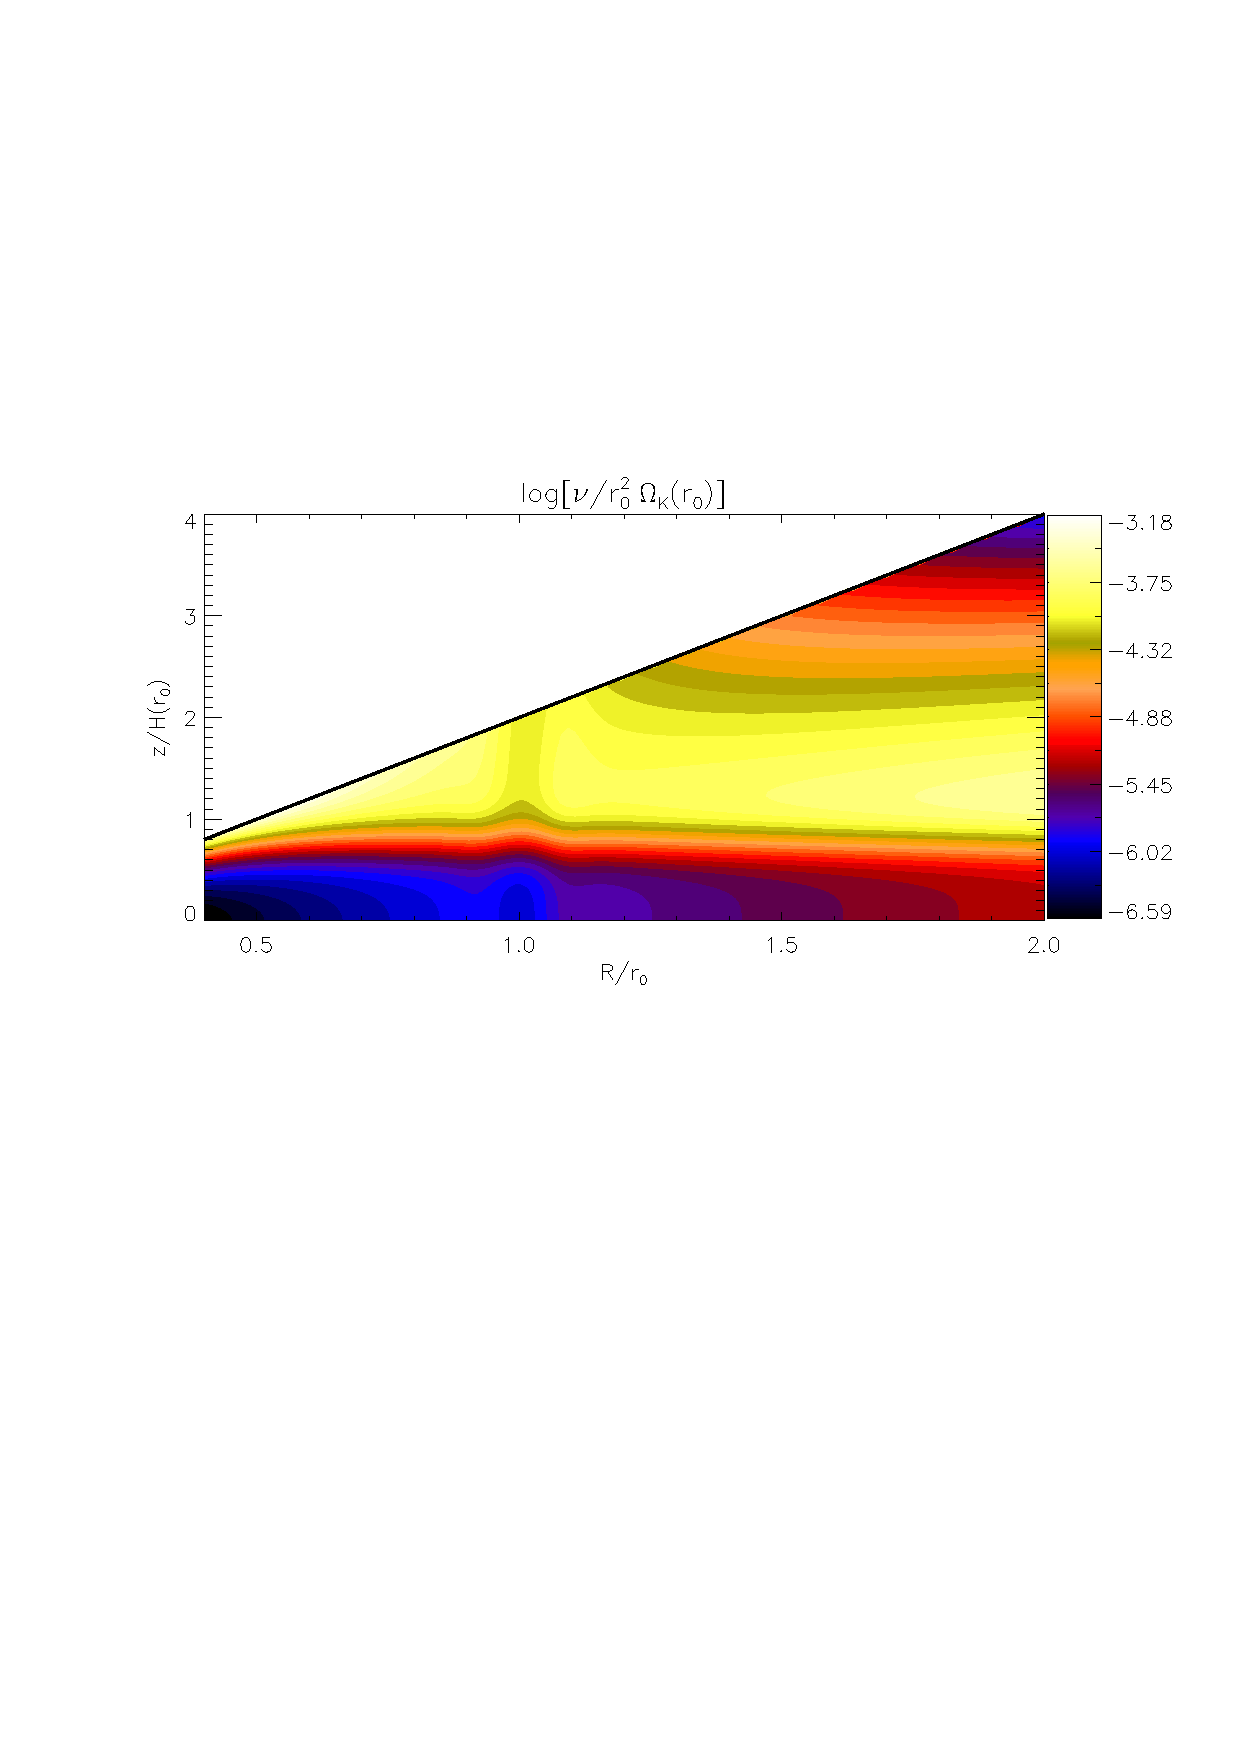
\includegraphics[width=\linewidth]{figures/pdisk_visc2d_layer2}
  \caption{Example of a two-layered kinematic viscosity profile
    resulting from Eq. \ref{visc_profile}. This specific plot
    corresponds to case V2. The solid line
    delineates the upper boundary of the computational domain.
    \label{visc2d}}
\end{figure}



\subsection{Simulations}
We consider discs with radial extent $[\rin,\rout]=[0.4,2.0]r_0$,
vertical extent with $n_h=2$ scale-heights and aspect-ratio $h=0.1$ at
$R=r_0$. We use $(N_r, N_\theta,
N_\phi)=(256,64,512)$ grid points. 
The resolution at the reference radius is then
$16,\,32,\,8$ cells per scale-height in $(r,\theta,\phi)$ directions,
respectively. The planetary potential is disabled for these runs
($M_p\equiv 0$).    

The bump parameters are set to $A=1.25$ and $\Delta R = 0.05r_0$ for
all runs in this section. The spherical radial velocity is subject 
to random perturbations of magnitude $10^{-4}c_s$ 
a few time-steps after initialisation. 

\subsubsection{Inviscid run}
For reference we simulate an effectively inviscid disc, case B0,
with the viscosity parameters $\hat{\nu}_0=10^{-9}$ and $A_\nu = 1$.  
The latter implies the viscosity is independent of $z$ at $R=r_0$.   
Inviscid setups similar to case B0 have previously been simulated
both in the linear and nonlinear regimes  \citep{meheut12, lin13}. So,
in addition to a control run, case B0 also serves to test the \pluto
code in simulating the RWI.    

\subsubsection{Viscous runs}
In these runs the floor viscosity is 
$\hat{\nu}_0=10^{-6}$. The control run case V0 has $A_\nu =
1$. Thus, case V0 is the viscous version of case B0.  
We then consider models where the kinematic viscosity increases by
a factor $A_\nu=100$ for $z>\zeta_\nu H_0$ at the bump radius. We
choose $\zeta_\nu=1.5,\,1.0$ for cases V1 and V2, respecively.  This gives a upper 
viscous layer of thickness $0.5H$ and $H$ at $R=r_0$. (See
Fig. \ref{visc2d} for a plot of the kinematic viscosity profile for case V2.) 
For case V1 and V2 the transition thickness is fixed to
$\Delta\zeta_\nu=0.2$.  
 
Finally, we consider a high viscosity run, case V3, with $\zeta_\nu =
0$, i.e. the viscous layer occupies the entire vertical domain. This
is equivalent to setting $\hat{\nu}_0=10^{-4}$ and $A_\nu=1$.  

\subsubsection{Linear growth rates and frequencies}
The present setup allows us to define a linear instability in the
usual way: exponential growth of perturbations measured with respect
to an axisymmetric steady equilibrium. A proper linear
stability analysis, including the full viscous stress tensor, is
beyond the scope of this paper, but we can nevertheless extract linear 
mode growth rates from the early evolution of the non-linear simulations.  

%For quantitative analysis of non-axisymmetric density structures, 
The $m^\mathrm{th}$ Fourier component of the density field is  
\begin{align}
\hat{\rho}_m(r,\theta,t) \equiv \int_0^{2\pi} \rho(\bm{r},t)\exp{(-\ii m\phi)}d\phi.
\end{align}
The magnitude of a Fourier mode is measured by 
\begin{align} 
a_m(t)\equiv \frac{b_m(t)}{b_0(0)},\quad b_m(t)\equiv \avg{|\hat{\rho}_m|}_r,
\end{align} 
where $\avg{\cdot}_r$ denotes averaging over a spherical shell (to be
chosen later). 
The complex frequency $\sigma_m$ associated with the $m^\mathrm{th}$ component 
is defined through 
\begin{align}\label{sigma}
  \frac{\p\hat{\rho}_m}{\p t} \equiv -\ii\sigma_m\hat{\rho}_m. 
\end{align}
The time derivative in Eq. \ref{sigma} can be computed implicitly by 
Fourier-transforming the continuity equation \citep[as done
  in][]{lin13}. 

%Note that we have defined the complex frequency as one would in a
%linear stability analysis because the RWI is a linear 
%instability. %% This definition is useful in assessing how the linear is
%% affected by the various boundary effects in the
%% linear phase (i.e. when perturbations are small). 
%The mode frequency defined here is therefore most appropriate to
%describe simulations where the axisymmetric background does not evolve
%in time (i.e. if $\p_t\avg{\rho}_\phi=0$), as required to define a
%linear instability. 

In a linear stability problem $\sigma_m$ is a constant eigenvalue. 
However, when extracted numerically from a non-linear simulation, 
we will generally obtain $\sigma_m=\sigma_m(r,\theta,t)$. Thus, we compute 
$\avg{\sigma_m}_r = m\omega_m + \ii q_m$    
where $\omega_m$ is the mode frequency and $q_m$ is the growth rate.
We normalise the linear frequencies by
$\Omega_0\equiv\Omega_i(r_0)\simeq\Omega_K(r_0)$. 

\subsection{Results}
Table \ref{artificial_bump} summarises the simulations presented in
this section. %, along with several diagnostic measures 
%of each case.  
 The linear mode frequencies are measured at 
$t=10P_0$ and averaged over the shell $r\in[0.8,1.2]r_0$.   
For convenience we will refer to $t\leq10P_0$ as the `linear
phase' since the relative density perturbations are
small ($\delta\rho\ll 1$) during this time.  
%The dominant azimuthal wavenumber is the mode with largest
%amplitude. 
The second set of measurements is made at $t=100P_0$, which is well
into the nonlinear regime. %The dominant mode is that with 
%$\mathrm{max}[a_m(100P_0)]$. 
The minimum Rossby number is measured at the midplane. 

\begin{table*}
  \centering
  \caption{Summary of hydrodynamic simulations initialized with a
    density bump. %% `UBC' is
    %% the boundary condition applied at the upper disc boundary. 
    Note that case V3
    is equivalent to setting 
    $\hat{\nu}_0=10^{-4}$ and $A_\nu=1$. \label{artificial_bump}}
  \begin{tabular}{lcccccl @{\extracolsep{0.1cm}} ccc}
    \hline\hline
    \multicolumn{4}{c}{\phantom{stuff}} &
    \multicolumn{3}{c}{$t = 10P_0$ (linear phase)}&
    \multicolumn{3}{c}{$t=100P_0$}\\
    \cline{5-7}\cline{8-10}
    Case  & $\log{\hat{\nu}_0}$ & $A_\nu$ &$\zeta_\nu$ & $m$ &
    $\omega_m/\Omega_0$ &
    $q_m/\Omega_0$ &  
    $m$ & $10^2a_m$ & $\mathrm{min}[Ro(z=0)]$ \\ 
    \hline
    B0 &-9 & 1 &n/a & 4 & 0.985  & 0.199  %omit = 3
    &  1 & 8.5  & -0.15   \\  
    
    V0  &-6 & 1 &n/a &  4 & 0.985  & 0.199   
    & 1 & 6.8 &  -0.11  \\
    
    V1  &-6 & 100 & 1.5  & 4 & 0.986  & 0.191
    &  1 & 7.8 &  -0.19 \\
    
    V2  & -6 & 100 & 1.0  &  4  & 0.986  & 0.182  
    &  1 & 4.9 &  -0.21 \\
    
    V3  & -6 & 100 & 0.0  &  4  & 0.986  &  0.131  
    &  3 &  3.7  &  -0.25 \\
   \hline
  \end{tabular}
\end{table*}

\subsubsection{Inviscid reference case}
Fig. \ref{bump0_bump1} 
shows the density fluctuation and Rossby number for
case B0. The dominant linear mode is $m=4$ with a growth rate
$0.2\Omega_0$. This 
corresponds to a growth timescale of $\sim P_0$. 
This is consistent with recent 3D linear calculations
\citep{meheut12,lin13}. Fig. \ref{bump0_bump1} shows that the
linear phase consists of non-axisymmetric vorticity perturbations on
either side of the density bump \citep{umurhan10}, i.e. vorticity
waves propagating along the PV gradients.     

The nonlinear outcome of the RWI is vortex-formation
\citep{li00}. Four vortices develop initially, but 
merge on a dynamical time-scale to produce 
a single vortex. %meheut12 vortex weakens on even longer time scales
                 %but we do not consider it here 
 Case B0 evolves similarly to previous numerical  
studies of the RWI in an inviscid disc
\citep[e.g.][where more detailed analyses are 
given]{meheut10,meheut12b}. This, together with the agreement with
previous linear simulations, demonstrates the ability of the \pluto
code to capture the RWI. 

\begin{figure}
  \centering
  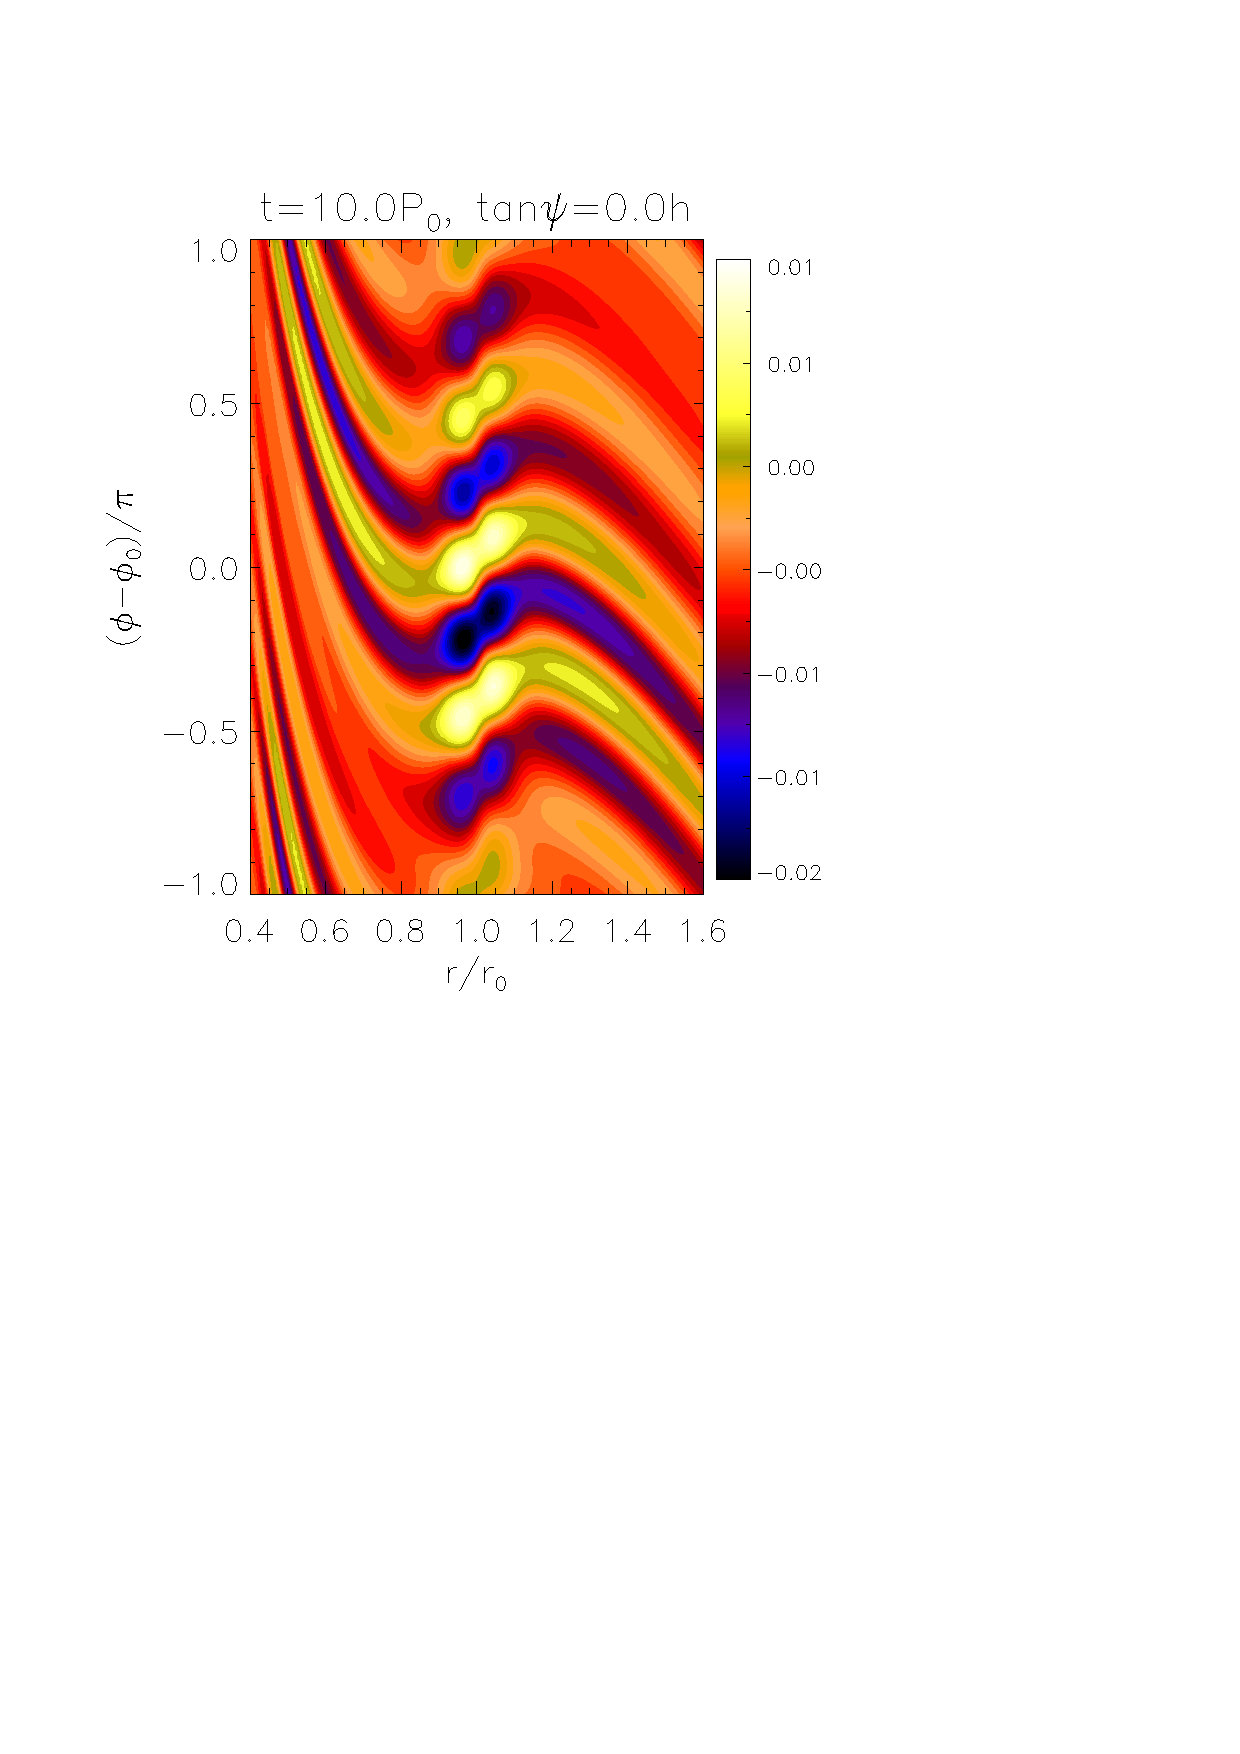
\includegraphics[scale=.27,clip=true,trim=0cm 0.9cm 0cm
    0cm]{figures/bump0_pdisk001}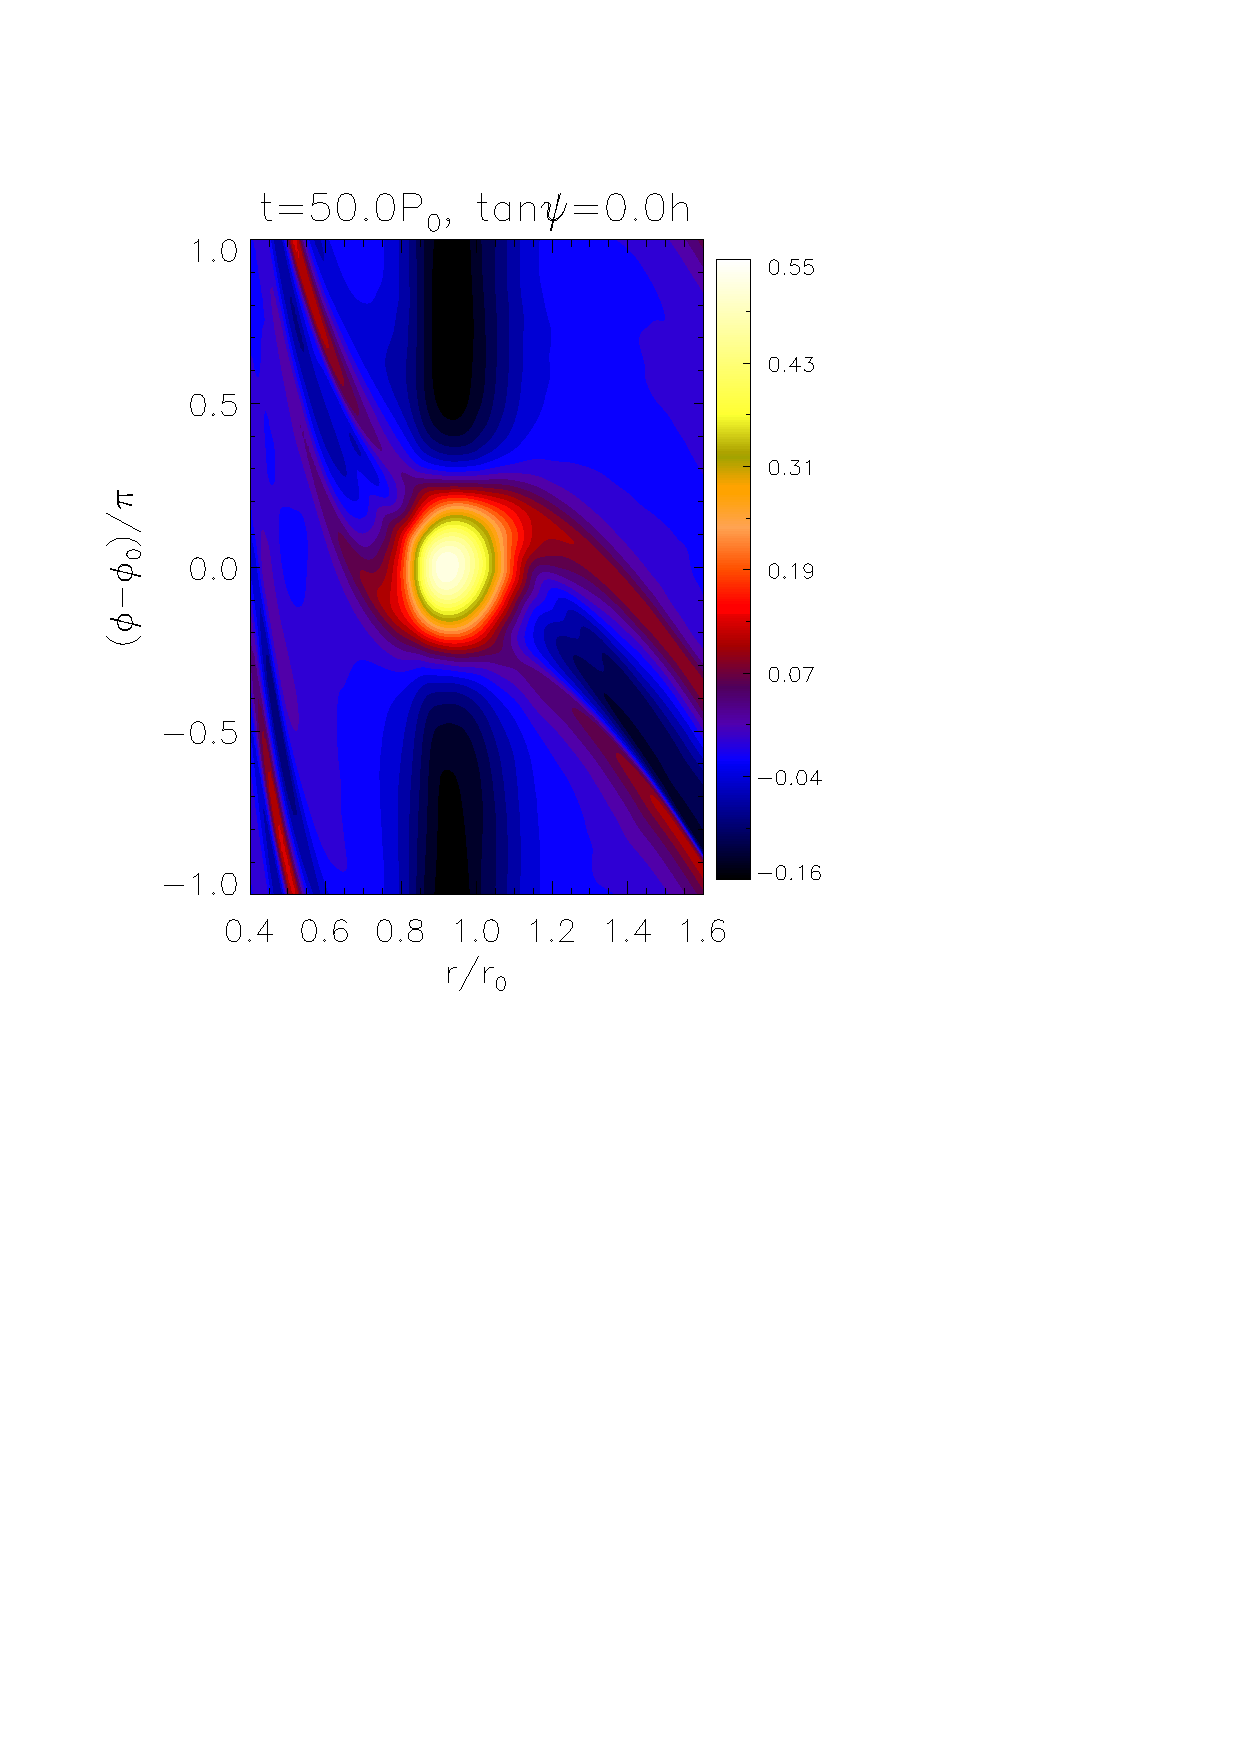
\includegraphics[scale=.27,clip=true,trim=2.3cm
    0.9cm 0cm
    0cm]{figures/bump0_pdisk005}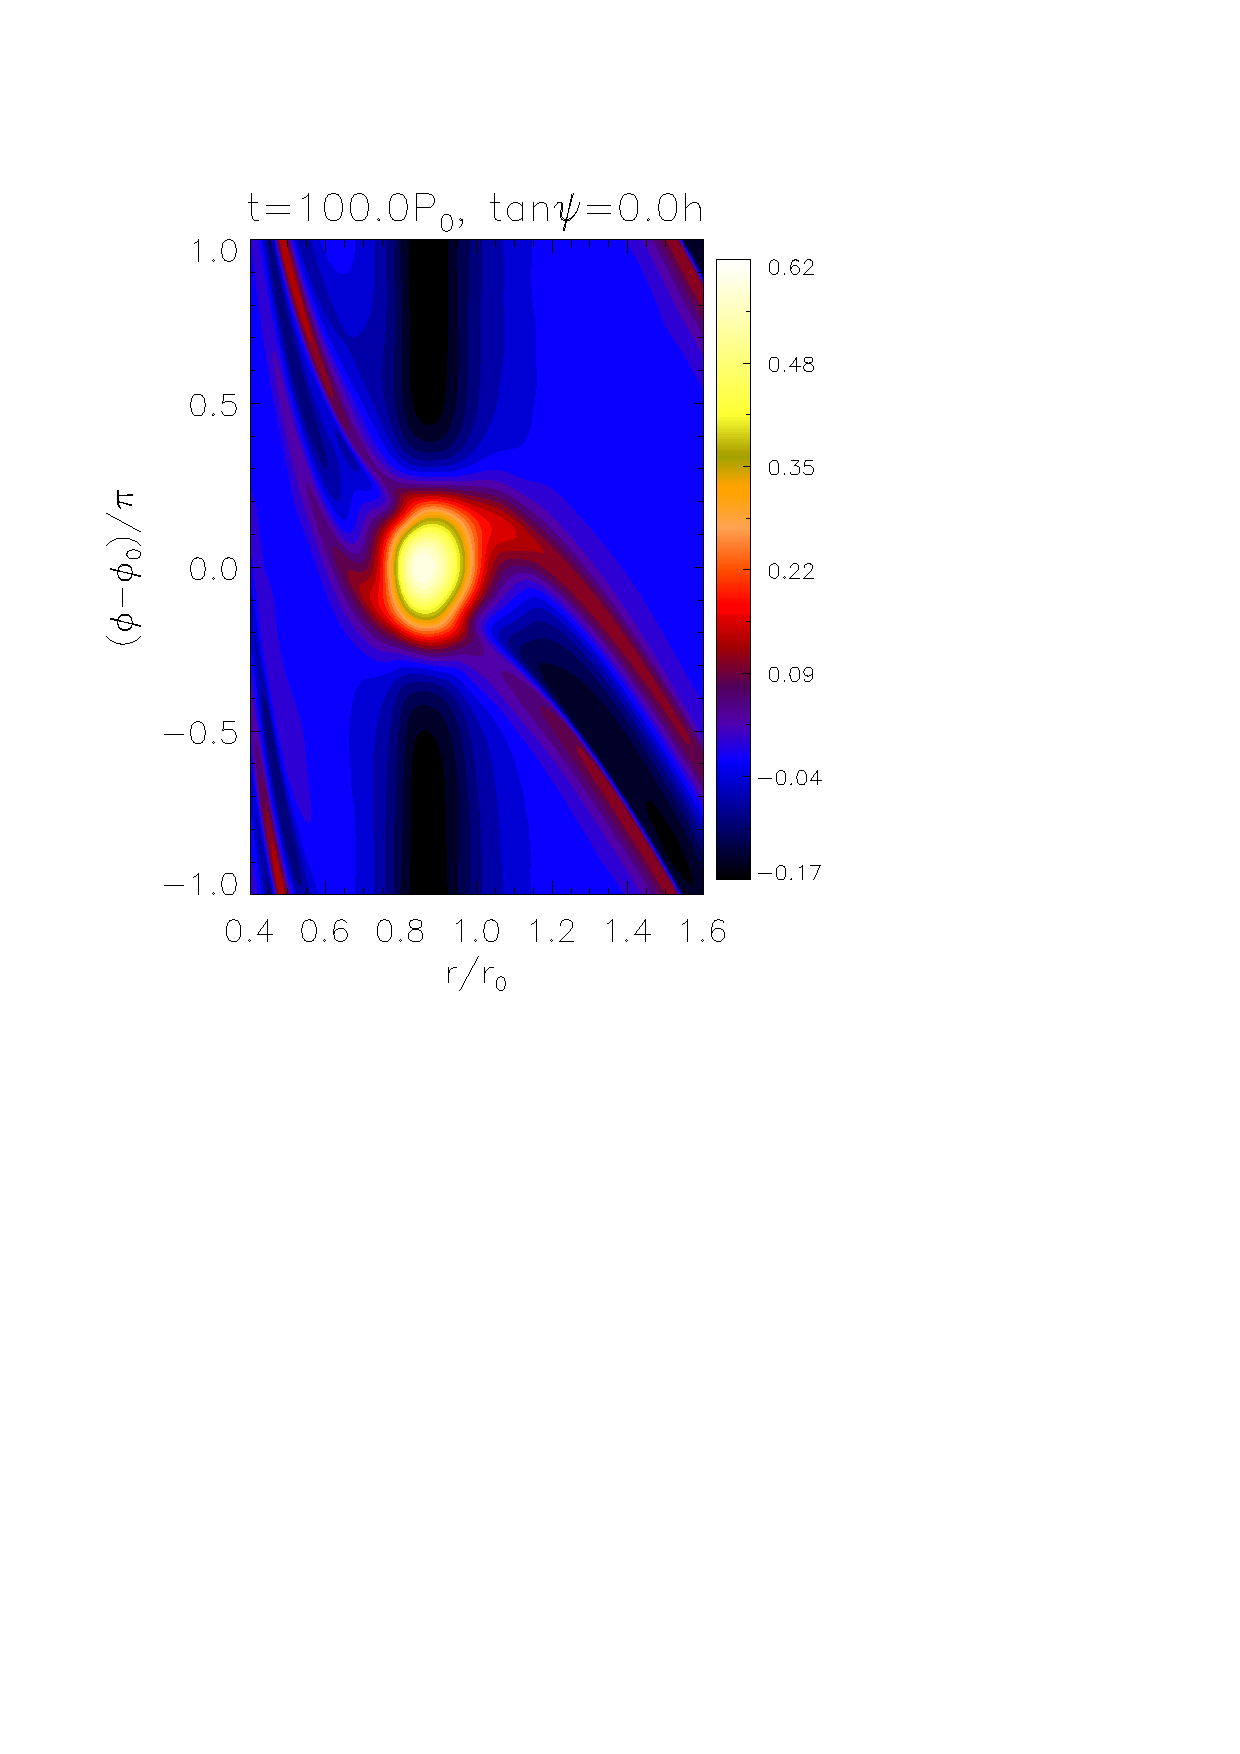
\includegraphics[scale=.27,clip=true,clip=true,trim=2.3cm
    0.9cm 0cm
    0cm]{figures/bump0_pdisk010}
   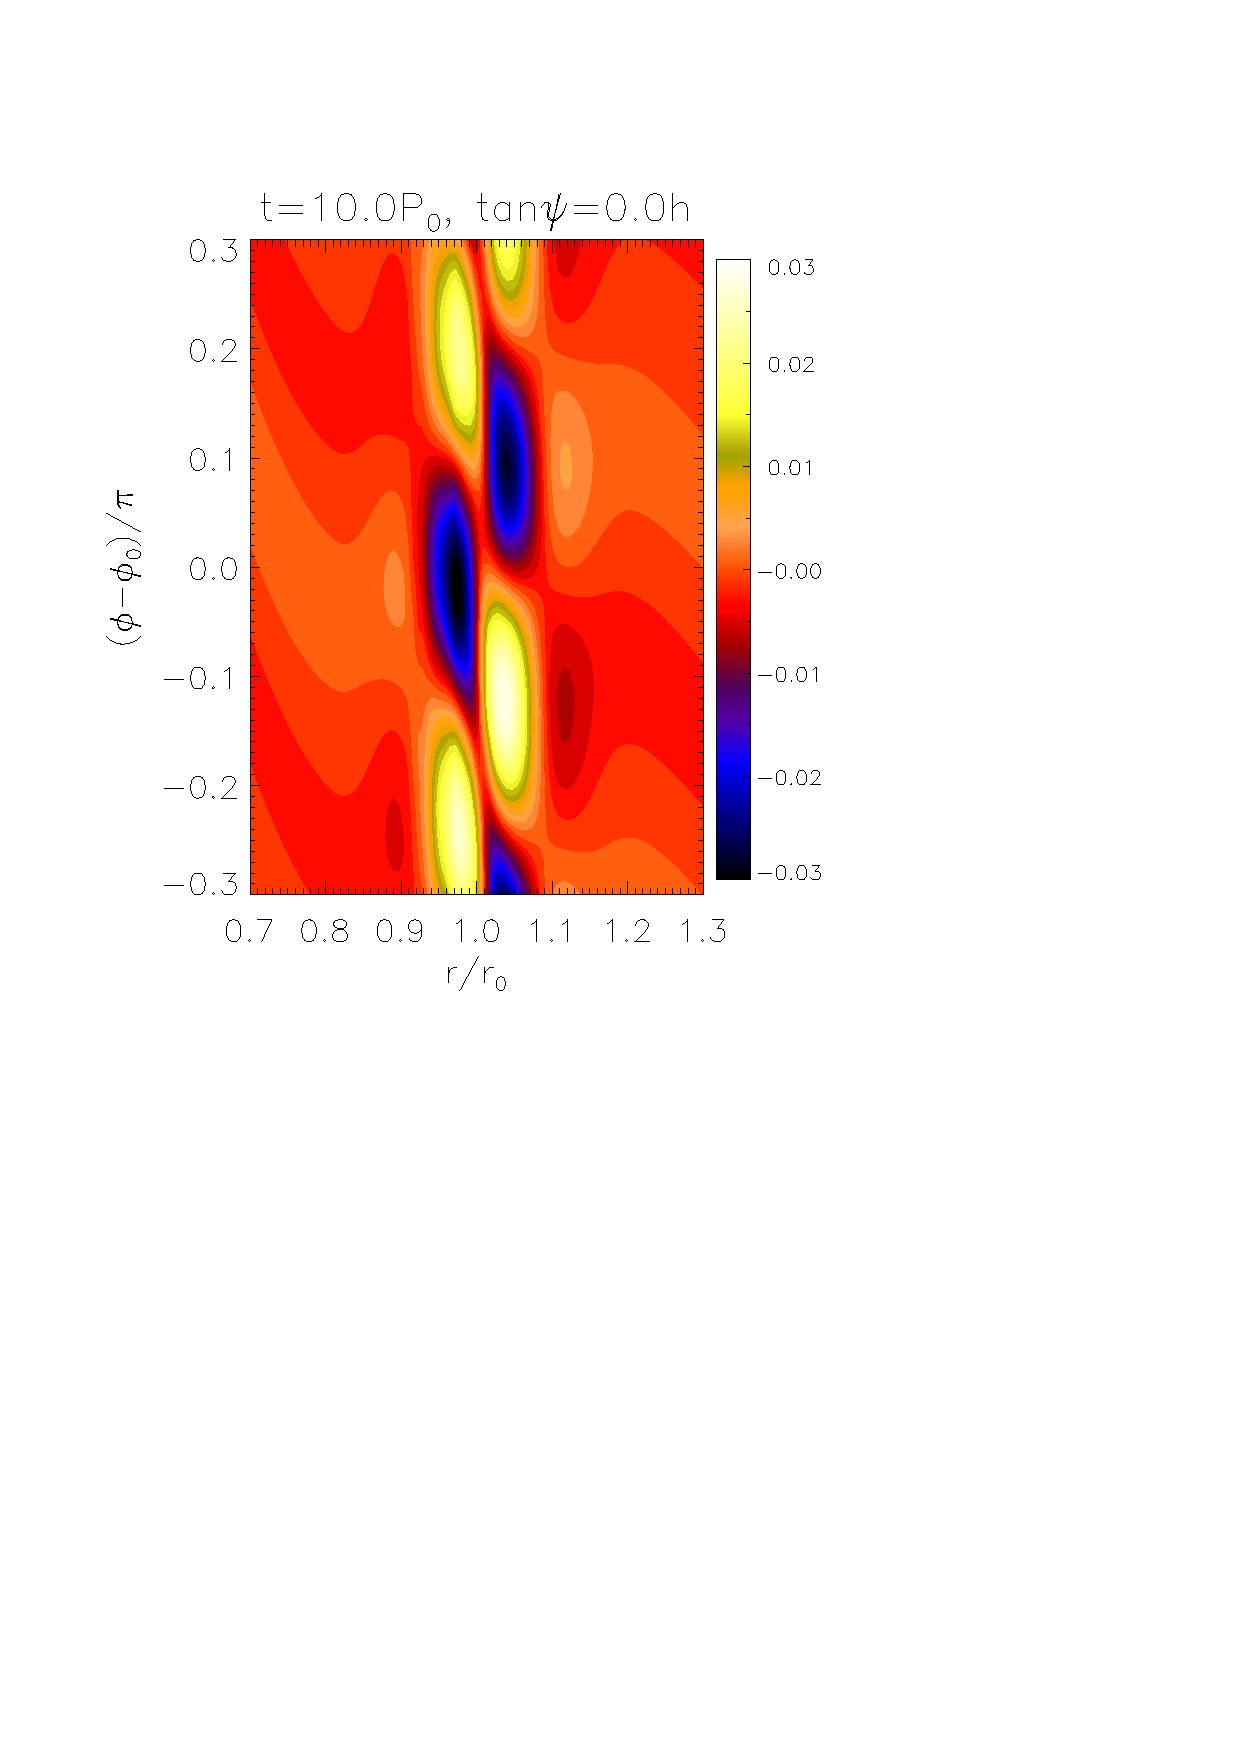
\includegraphics[scale=.27,clip=true,trim=0cm 0.cm 0cm
     0.9cm]{figures/bump0_vort001}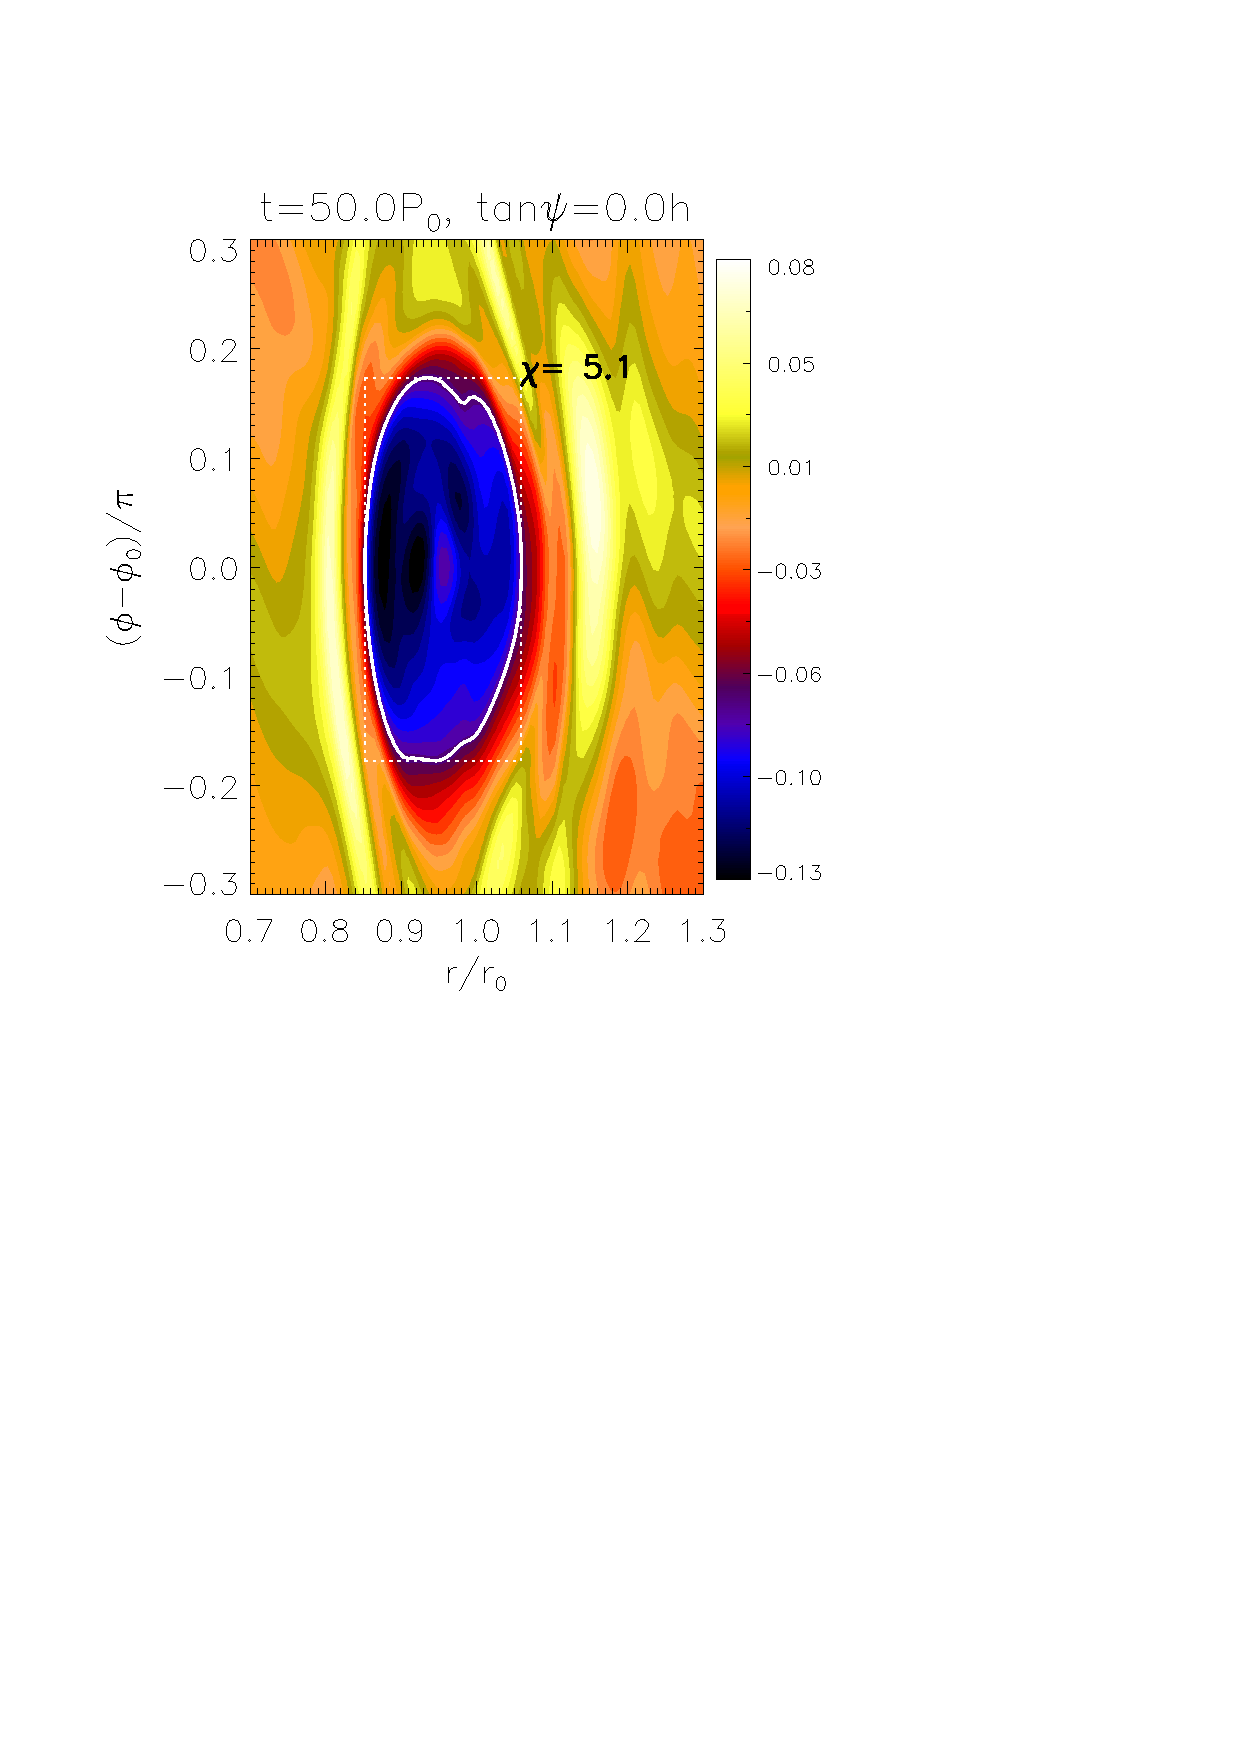
\includegraphics[scale=.27,clip=true,trim=2.3cm
     0.cm 0cm
     0.9cm]{figures/bump0_vort005}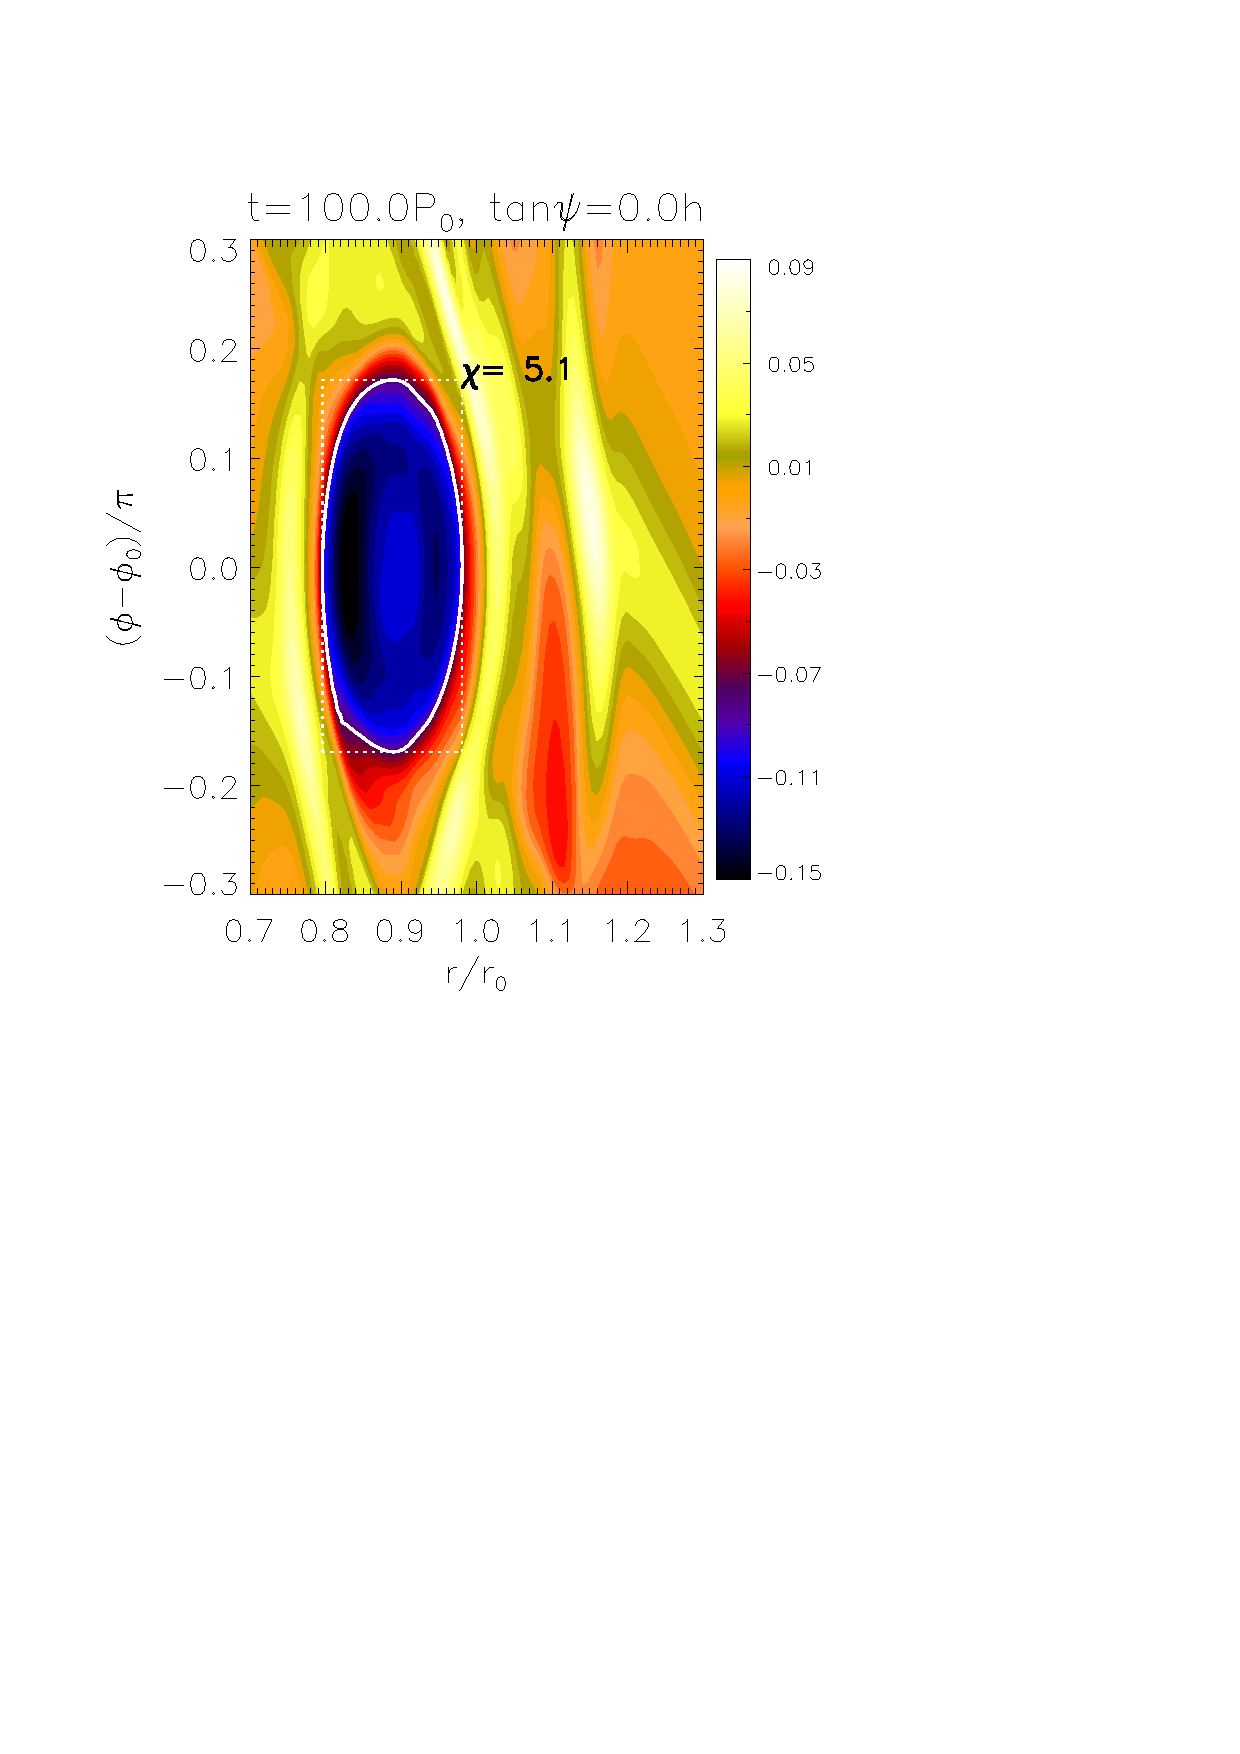
\includegraphics[scale=.27,clip=true,clip=true,trim=2.3cm
     0.cm 0cm
     0.9cm]{figures/bump0_vort010}
  \caption{Evolution of the inviscid case B0. Top: midplane density fluctuation, 
    $\Delta\rho(z=0)$. Bottom: midplane
    Rossby number (note the different axis range from the top plots). 
    Here, $\chi$ is an empirical measure of the final vortex
    aspect-ratio. $\phi_0$ is the azimuth of 
    $\mathrm{max}\left[|\Delta\rho(z=0)|\right]$
    \label{bump0_bump1}}
\end{figure}

\subsubsection{The effect of a viscous layer}
We now examine viscous cases V0 --- V3. Recall  
from Table \ref{artificial_bump} that the 
thickness of the upper viscous layer increases from case V0 to case
V3. At the reference radius, the viscous layer (with $
\hat{\nu}\sim10^{-4}$) occupies the uppermost $0\%,\,25\%,\,50\%$ and
$100\%$ of the vertical domain for cases V0, V1, V2 and V3,
respectively.    

We first compare the control case V0 to the fiducial
inviscid case B0. Table \ref{artificial_bump} shows that despite
increasing the viscosity by a factor of $10^3$, the change to the
linear mode frequencies are negligible in going from case B0 to
V0. The value of $a_m$ and minimum Rossby number show that the final
vortex in V0 is only slightly weaker than that in B0. This is also
reflected in  Fig. \ref{bump0_bump1} (case B0) and the left most column of
Fig. \ref{vdamp0} (case V0). Case V0 develops a more elongated 
vortex with smaller $|\Delta\rho|$ than that in case B0. 
  
As we increase the thickness of the viscous layer from case V0 to V3, 
Table \ref{artificial_bump} shows the dominant linear mode remains at
$m=4$, but linear growth rate does appreciably decrease 
(by $\sim 34\%$ from case V0 to V3). However, these linear growth timescales
are still $O(P_0)$.  
We thus have the important result that the effect of viscosity
(layered or not) on the
instability through the linear perturbations is not significant as the
RWI remains dynamical even in the high viscosity disc.   %linear
                                %perturbations not effecitvely damped out

The top row of Fig. \ref{vdamp0} shows that layered viscosity has a
non-trivial effect on $\Delta\rho$ in the
non-linear regime. $|\Delta \rho|$ increases
from case V0 to V1, then decreases from cases V1 to V3 (but aquires a
more global distribution). The dominant azimuthal wavenumber also
increase: vortices do not readily merge in case V2 and V3. 
 
%(third and fourth columns in the top row of Fig. \ref{vdamp0}).  
%While
%$\max(\Delta\rho)$ decreases with increasing viscosity, its
%distribution becomes more global.  

%replace with energy discussion 
%The top row of Fig. \ref{vdamp0} show the density fluctuations of the
%viscous cases. Comparing the second column in Fig. \ref{vdamp0} (case
%V1) to the top panel (case V0), we see that introducing the
%viscous layer lengthens the lifetime of the density perturbation in the
%nonlinear regime, since $\max(\Delta\rho)\simeq 0.47$ is maintained for
%the second half of the simulation for case V1, but this value decreases
%by about 0.1 for case V0 over the same timescale. 

%Increasing the viscous layer further to case V2 and V3, we observe an
%increase in the dominant azimuthal wavenumber in the nonlinear phase
%(third and fourth columns in the top row of Fig. \ref{vdamp0}).  
%While
%$\max(\Delta\rho)$ decreases with increasing viscosity, its
%distribution becomes more global.  

\begin{figure*}
   \centering
   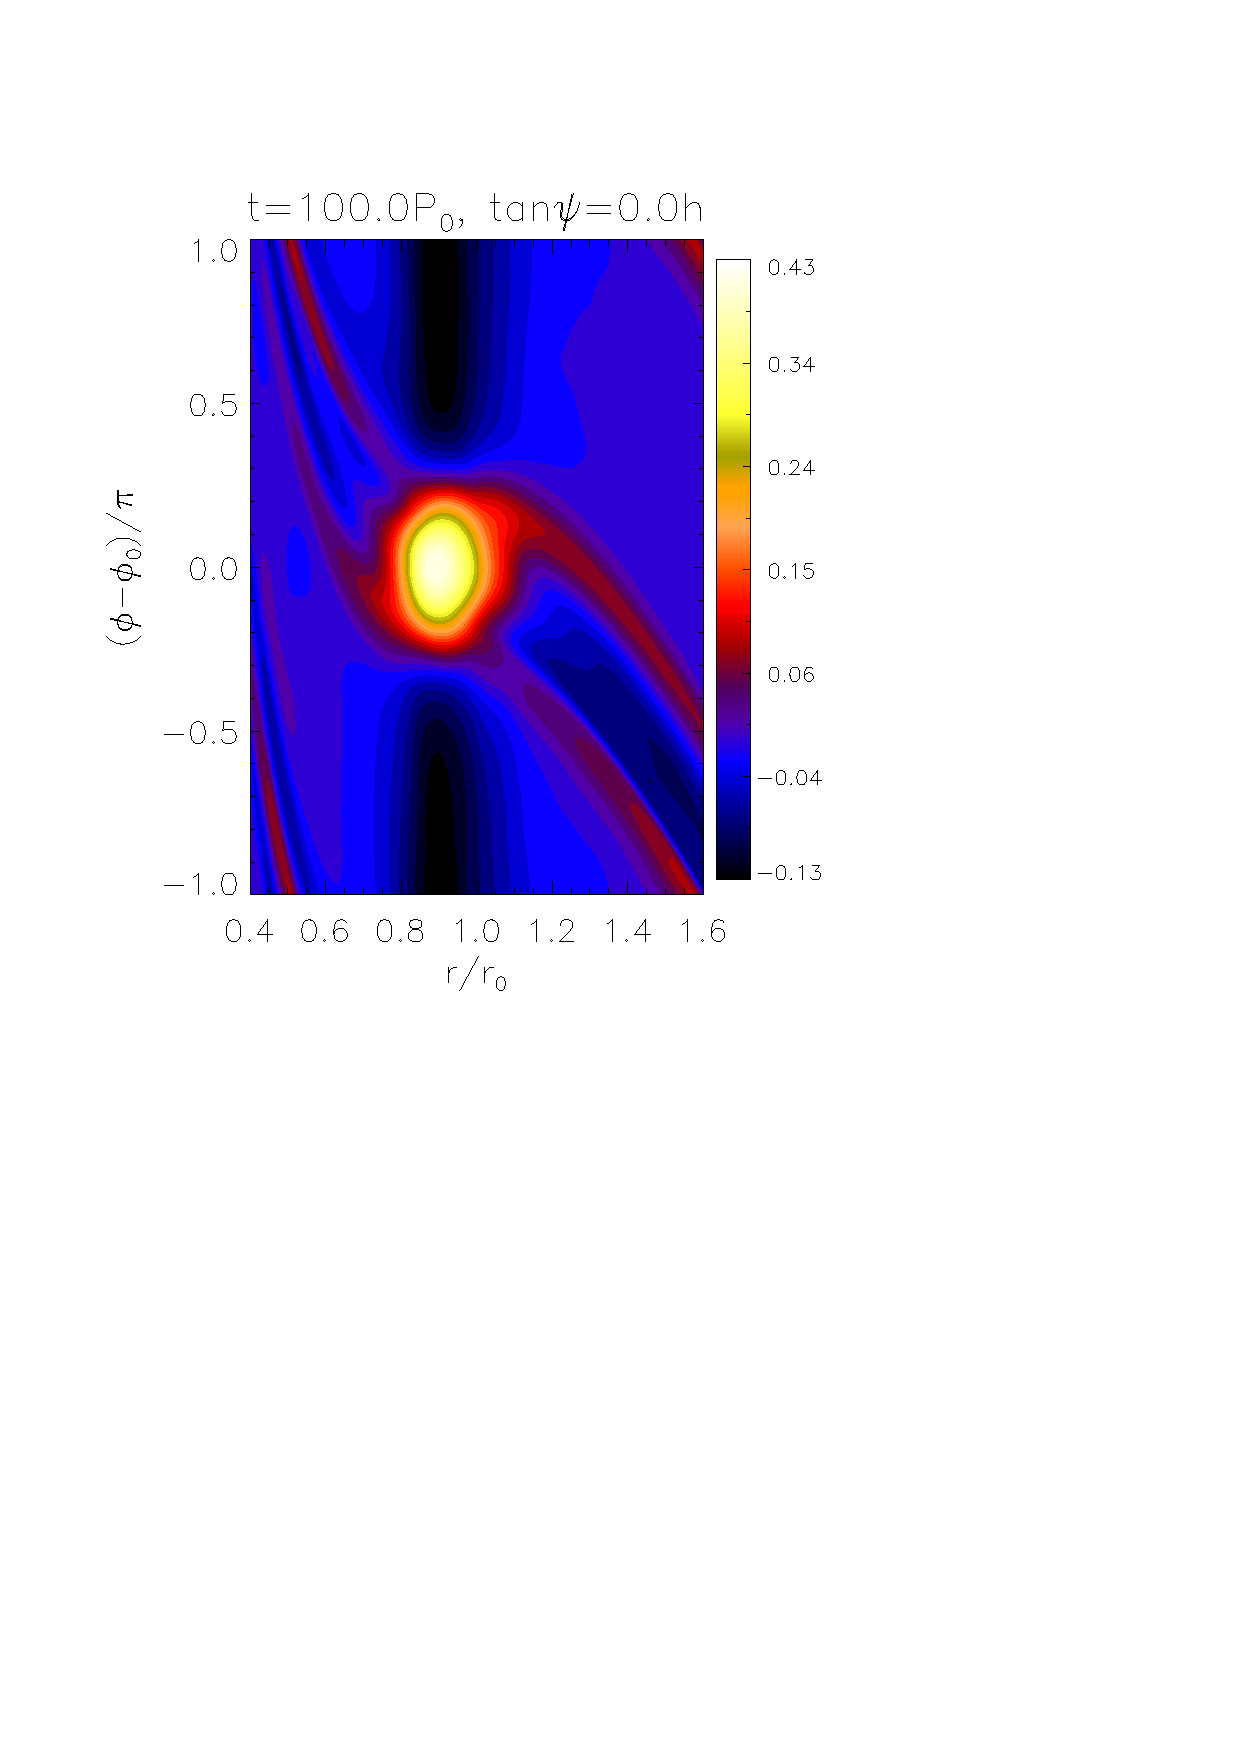
\includegraphics[scale=.43,clip=true,trim=0cm 0.9cm 0cm
     0.99cm]{figures/vdamp0_pdisk010}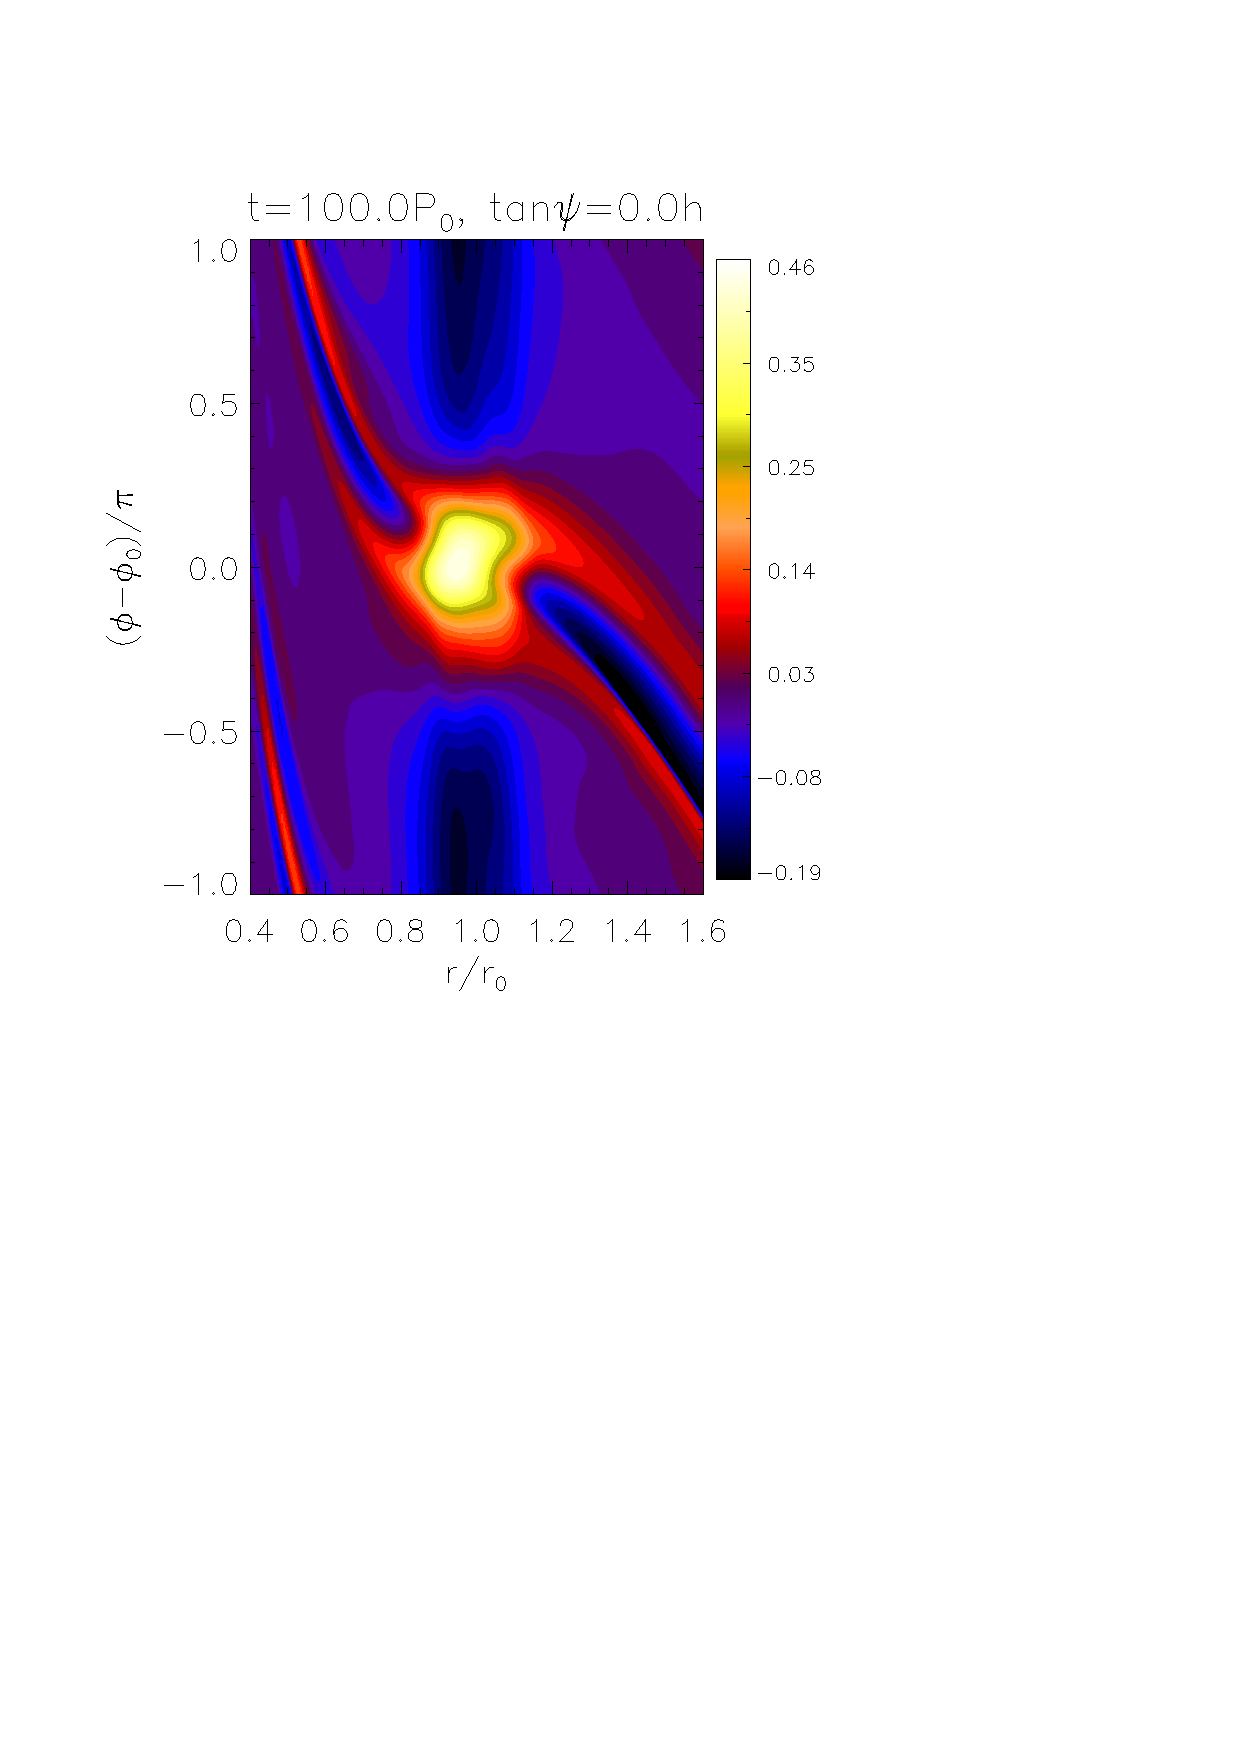
\includegraphics[scale=.43,clip=true,trim=2.3cm
     0.9cm 0cm
     0.99cm]{figures/vdamp2_pdisk010}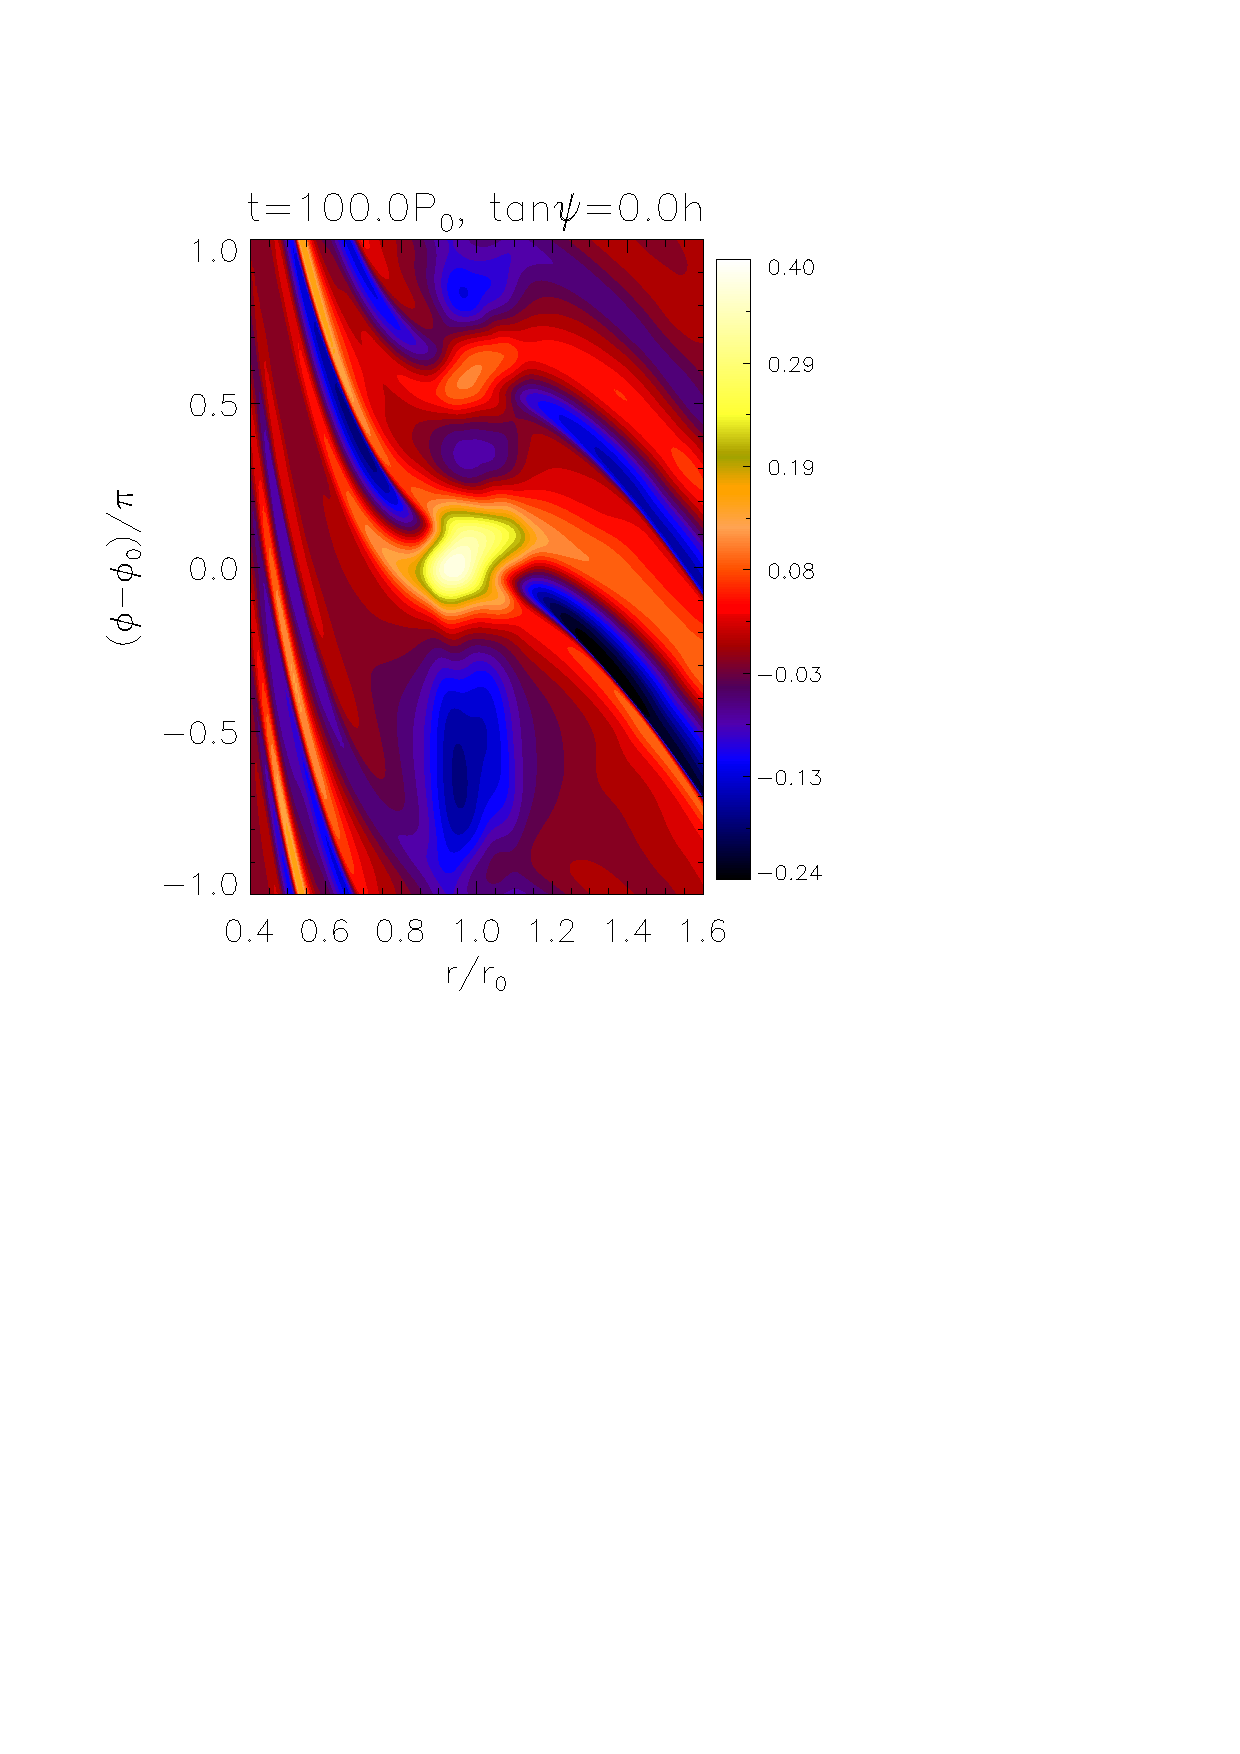
\includegraphics[scale=.43,clip=true,trim=2.3cm 
     0.9cm 0cm
     0.99cm]{figures/vdamp3_pdisk010}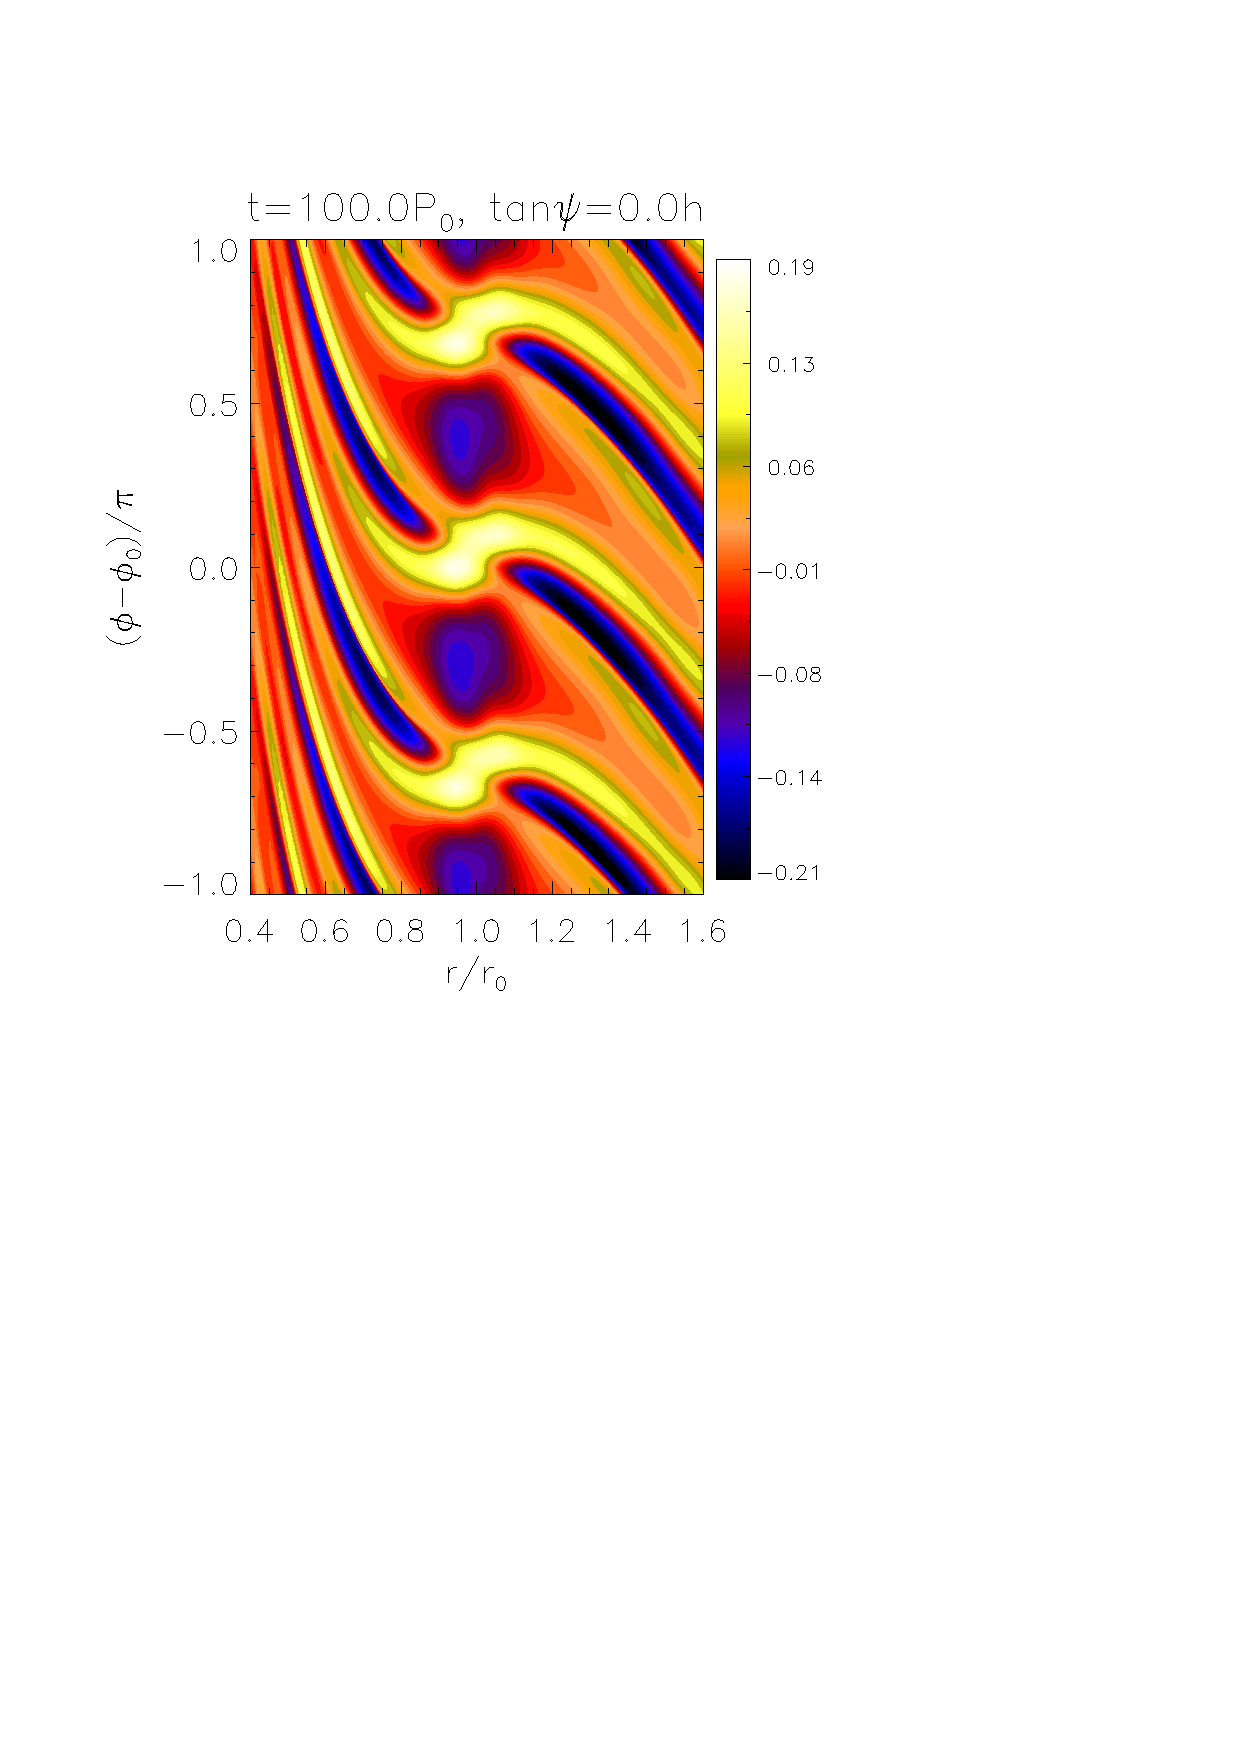
\includegraphics[scale=.43,clip=true,trim=2.3cm
     0.9cm 0cm
     0.99cm]{figures/vdamp0_nu4_pdisk010}\\
      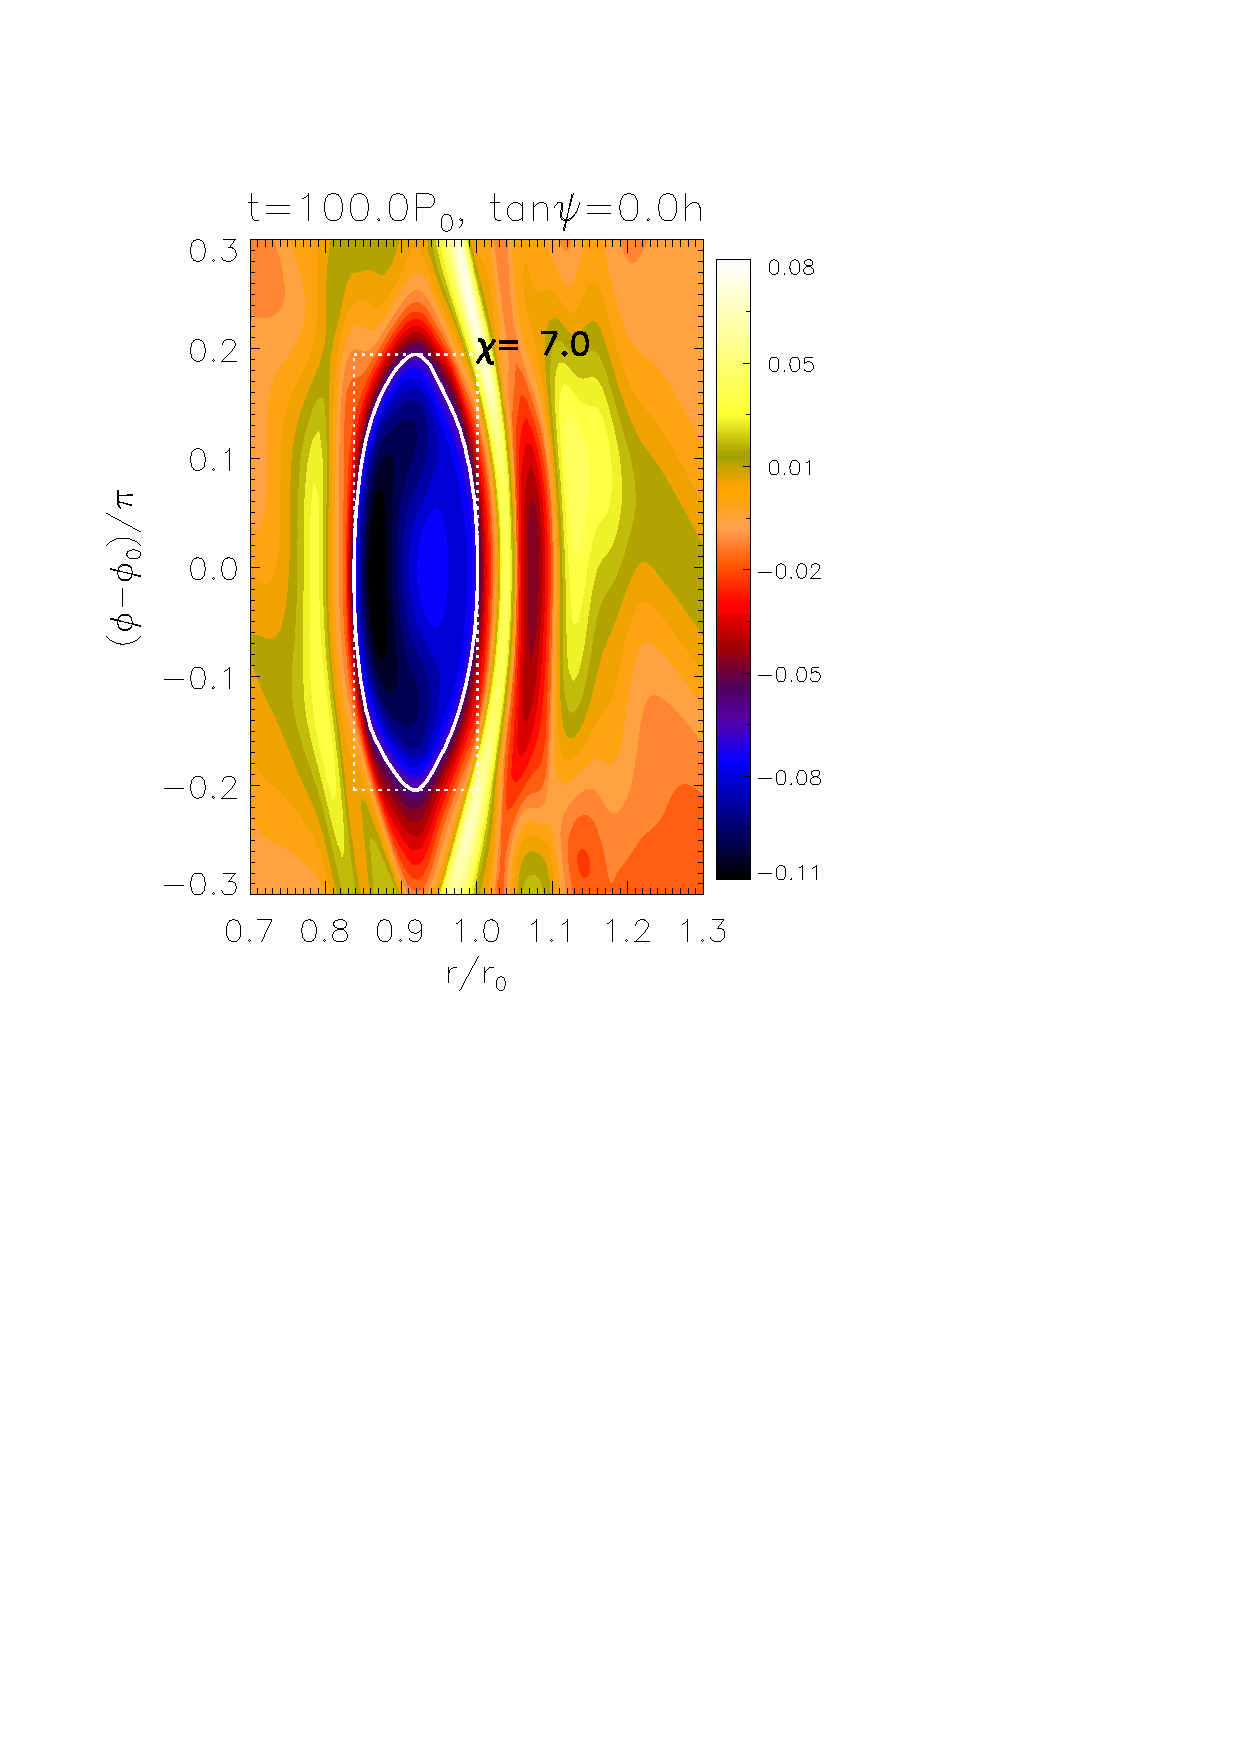
\includegraphics[scale=.43,clip=true,trim=0cm 0.cm 0cm
     0.99cm]{figures/vdamp0_vort010}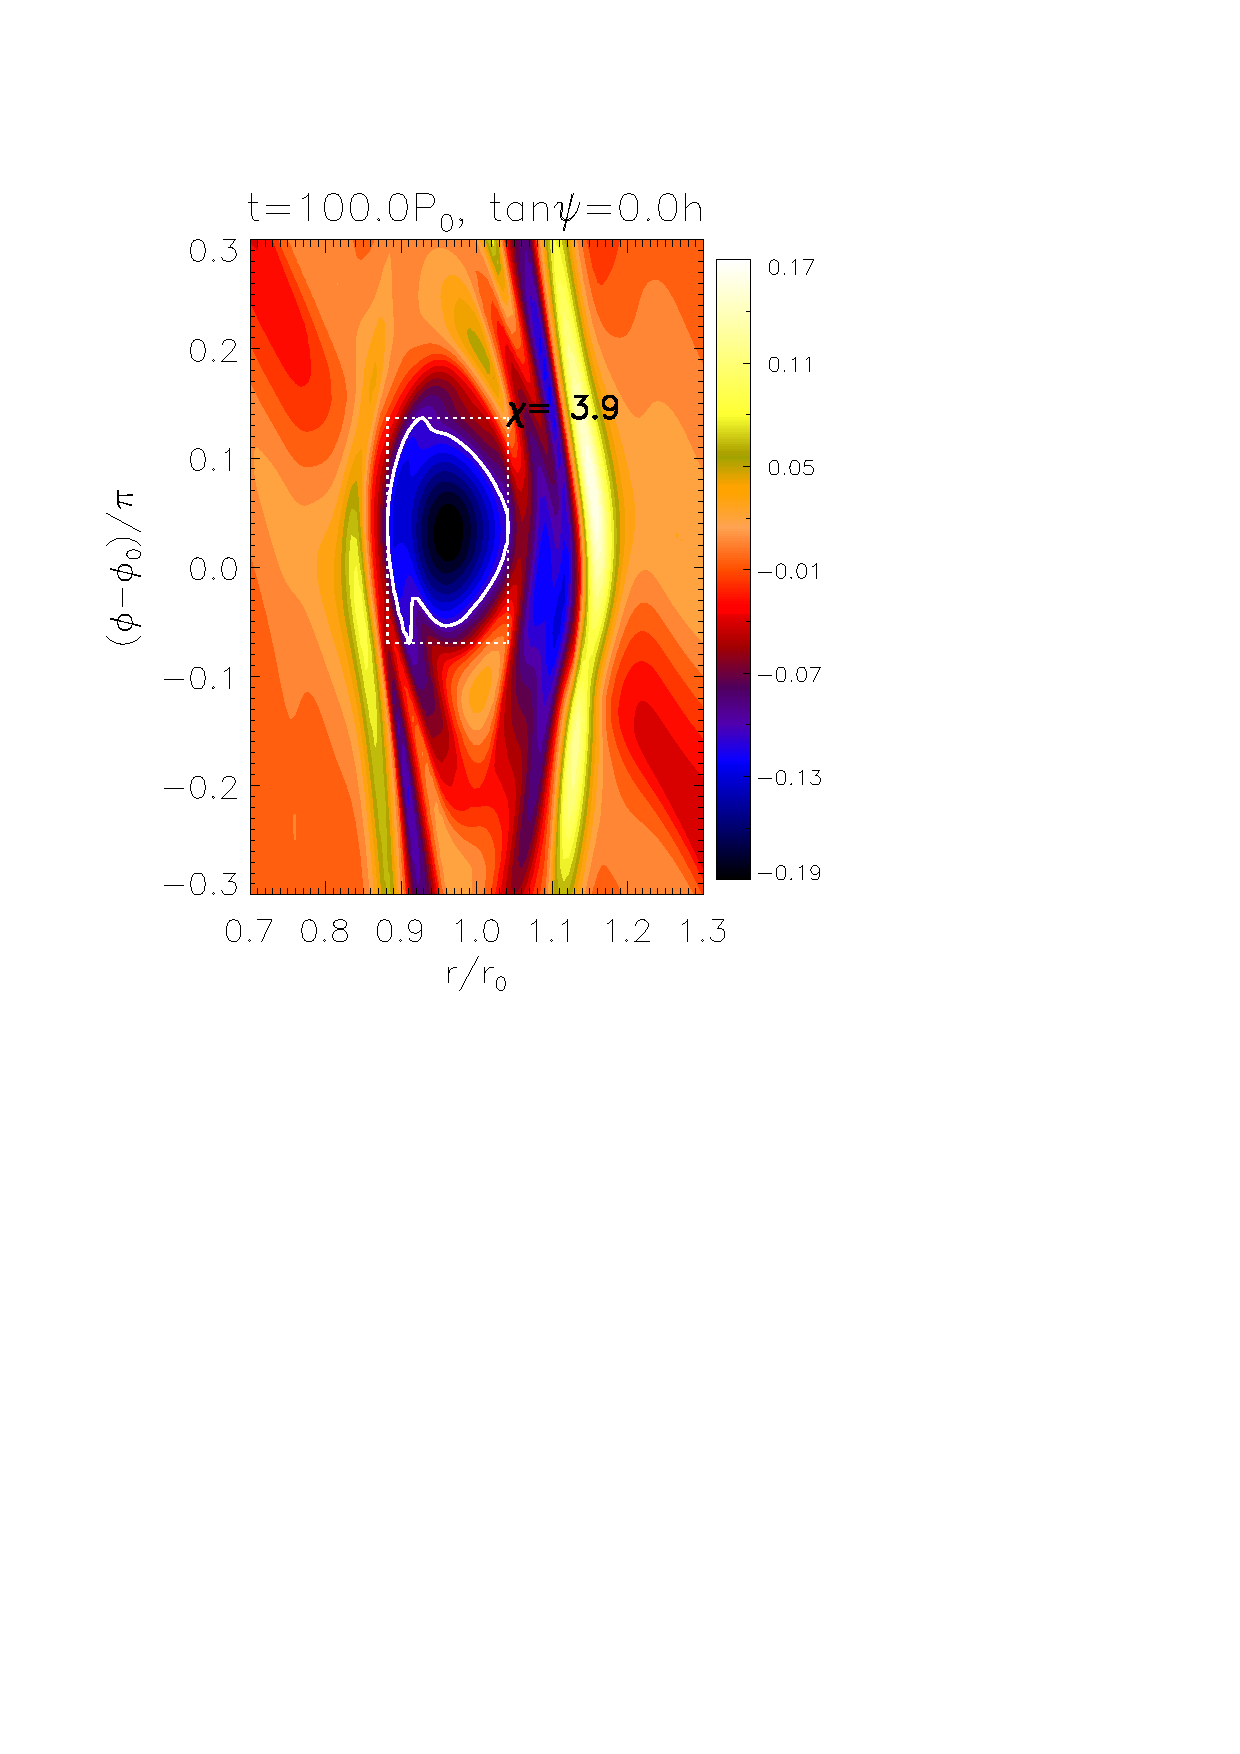
\includegraphics[scale=.43,clip=true,trim=2.3cm
     0.0cm 0cm
     0.99cm]{figures/vdamp2_vort010}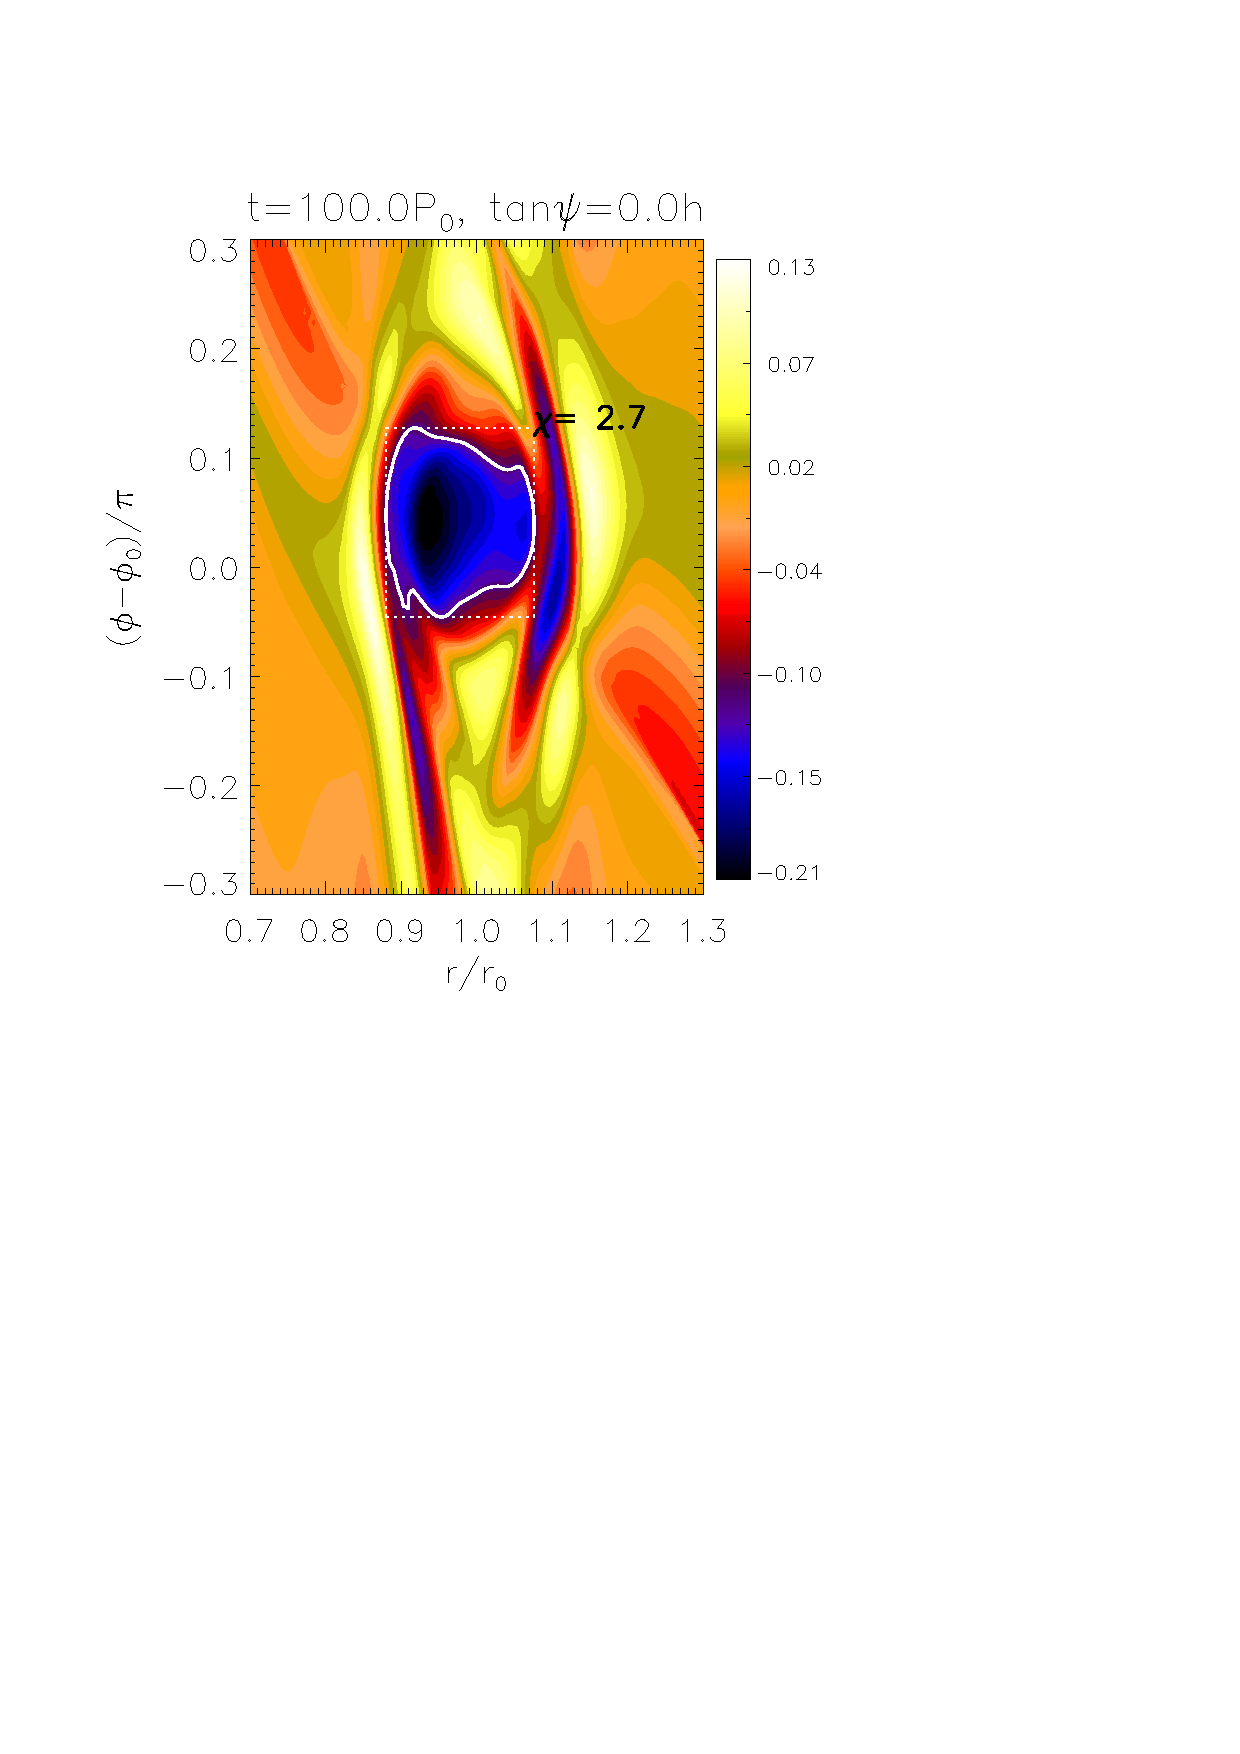
\includegraphics[scale=.43,clip=true,trim=2.3cm 
     0.0cm 0cm
     0.99cm]{figures/vdamp3_vort010}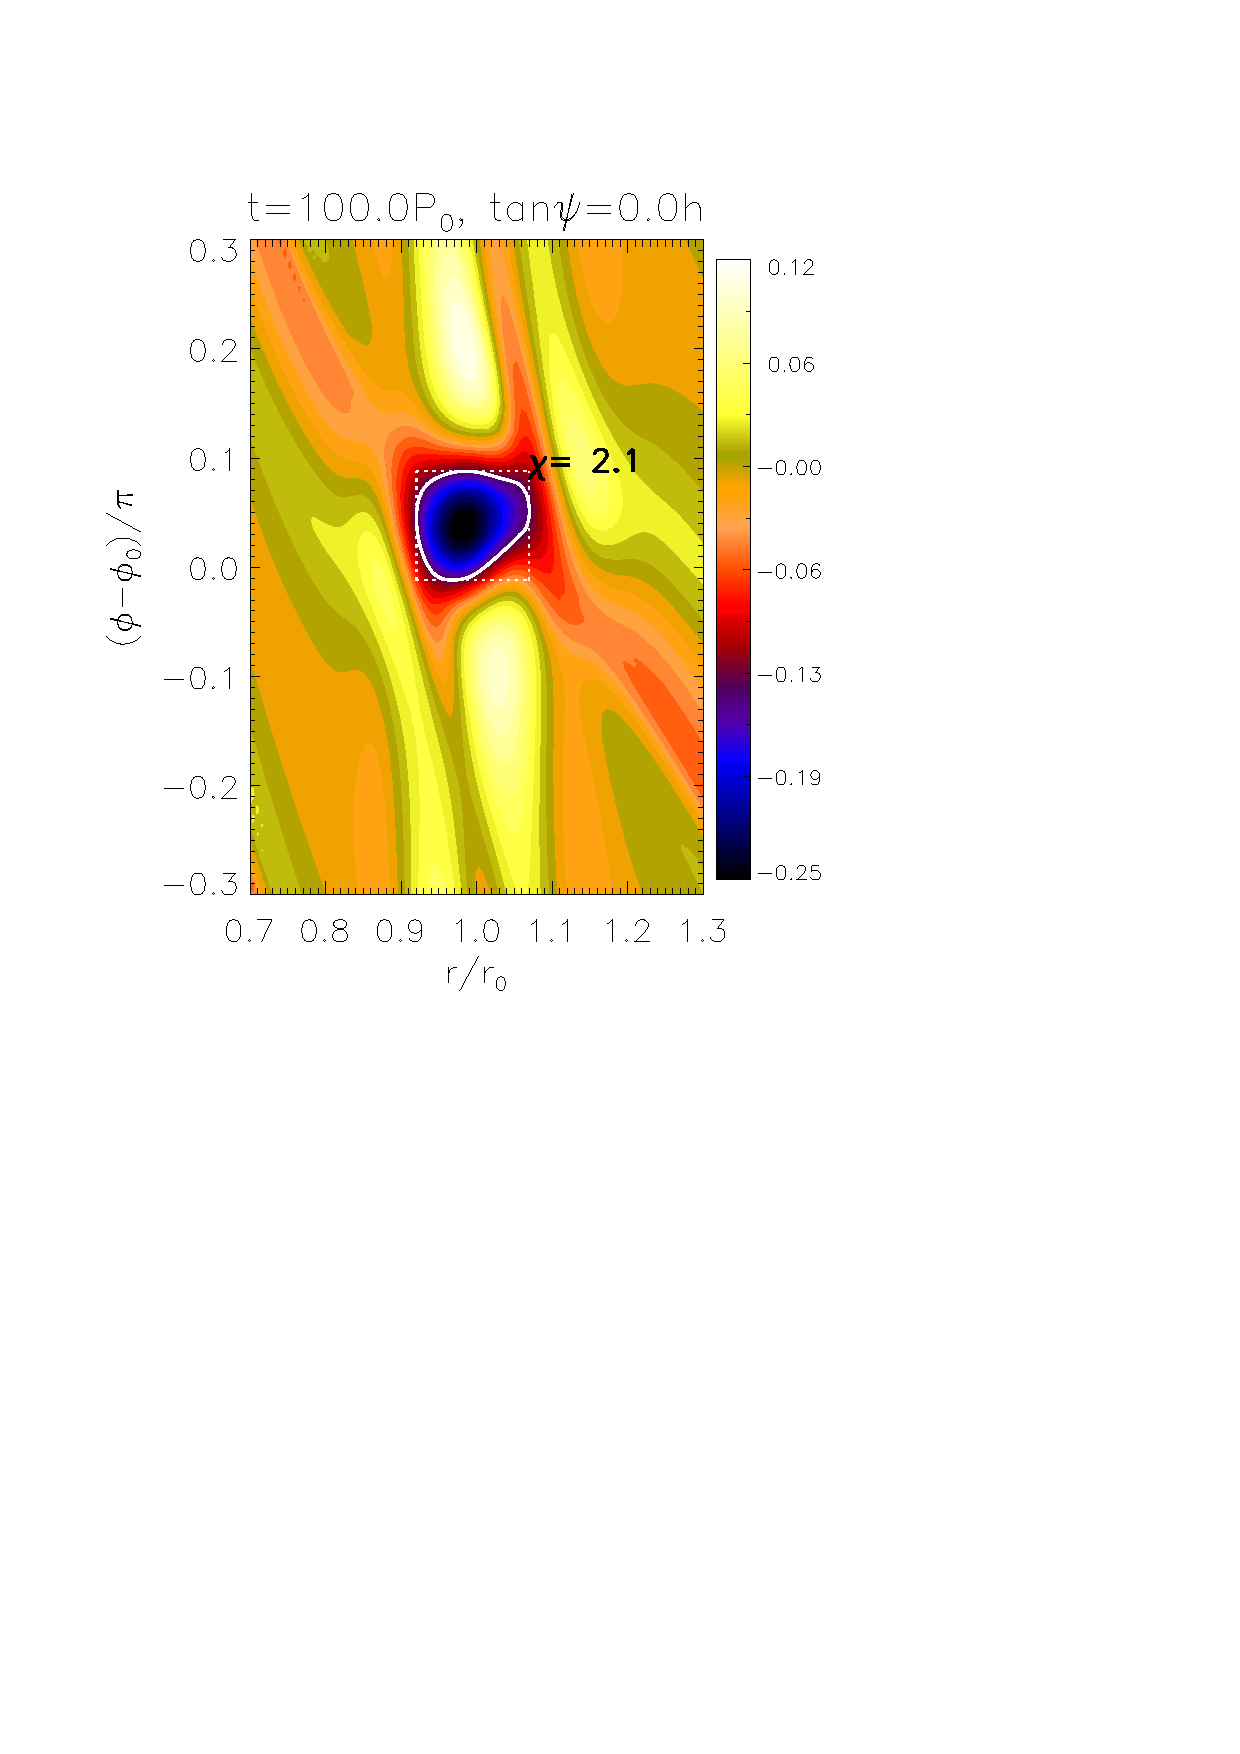
\includegraphics[scale=.43,clip=true,trim=2.3cm
     0.0cm 0cm
     0.99cm]{figures/vdamp0_nu4_vort010}
   \caption{Vortex formation in viscous discs initialised with
     artificial density bumps. Snapshots are taken at $t=100P_0$. The
     thickness of the viscous layer increases from left to 
     right: case V0, V1, V2 and V3.   
     Top: non-axisymemtric density field at the midplane
     $\Delta\rho(z=0)$. Bottom: midplane Rossby number
     $Ro(z=0)$. Here, $\phi_0$ is the azimuth of $\max[\Delta\rho(z=0)]$. 
     \label{vdamp0}
   }
\end{figure*}

The bottom row of Fig. \ref{vdamp0} compares the Rossby number
associated with the over-densities. Thickening the viscous 
layer decreases the vortex aspect ratio. Since their widths remain
at $\sim 2H_0$, the vortices become smaller with increasing
viscosity. This may be partly attributed to fewer vortex merging
events having occured as viscosity is increased. The merging of
two vortices usually leads to a larger but weaker vortex (smaller
$|Ro|$), so if vortex merging is resisted then each vortex may evolve
separately. Strangely, vortices become stronger  (more negative $Ro$)
as viscosity is increased.

We compare  in Fig. \ref{bump_energy} the perturbed kinetic energy for 
cases B0, V0 and V1; which are all dominated by a single vortex in 
quasi-steady state. Thus we compute $W_1$, and
average it over the atmosphere ($\tan{\psi}\in[0,0.5]h$) and the 
disc bulk ($\tan{\psi}\in[0.5,2.0]h$). These averages are restricted
to the vortex region $r\in[0.8,1.2]r_0$. Note that for the layered
case V1, the distinction between disc bulk and atmosphere also
separates the low and high viscosity regions, respectively. 
%In an averaged sense, among 
%these runs case B0 has the lowest viscosity while case V1 has the
%highest.

Fig. \ref{bump_energy} displays only a minor difference between the
perturbed kinetic energy densities between the disc bulk and
atmosphere, even in case V1 where the viscosity in the two regions
differ by 100. This suggests that the perturbation evolves
two-dimensionally. The energy in case B0 and V0 are both subject to
slow decay. By contrast case V1, which has the highest viscosity in an
averaged sense, does \emph{not} show such a decay. This suggests that
viscosity could in fact strengthen the perturbation. 

\begin{figure}
  \centering
  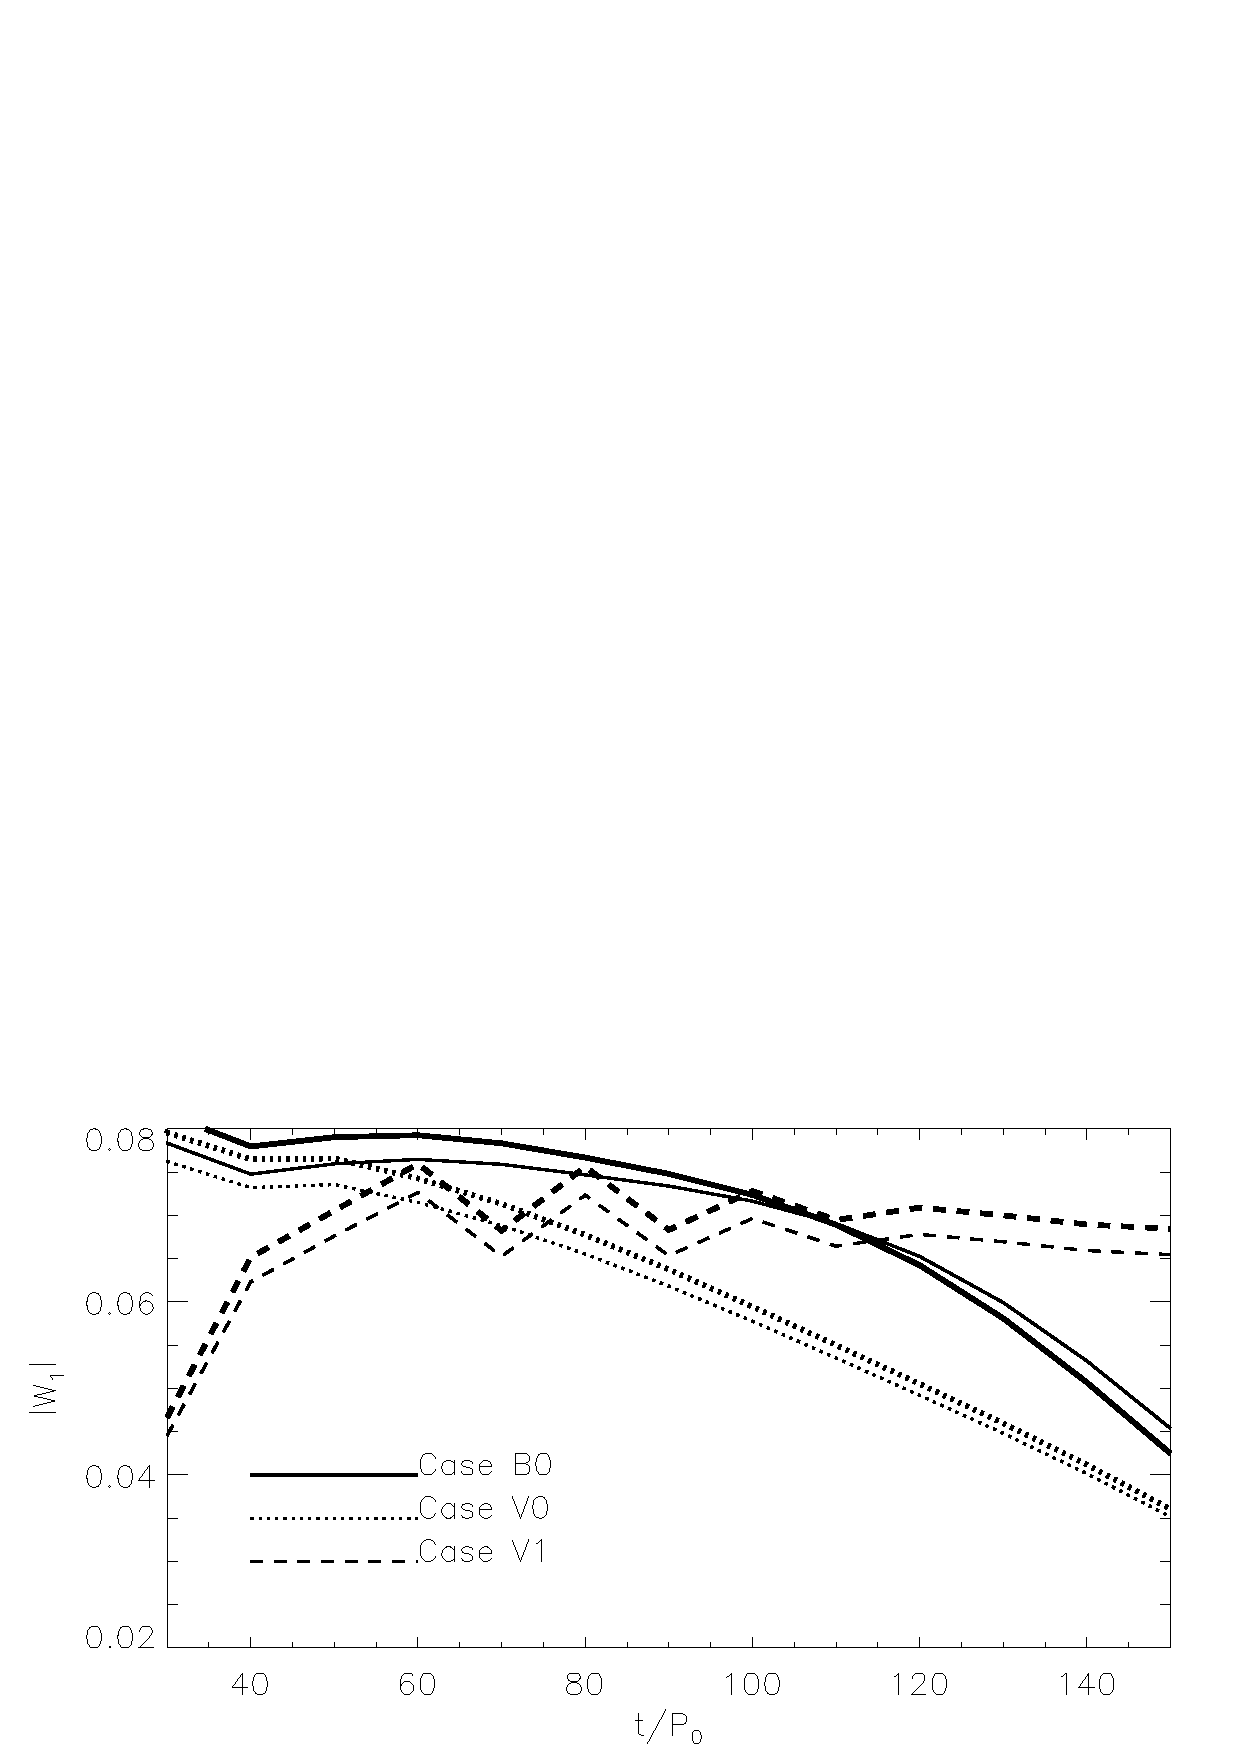
\includegraphics[width=\linewidth]{figures/pdisk_kerz_cases_bump}
  \caption{The $m=1$ component of the kinetic energy density for
    the inviscid case B0 (solid), low viscosity case V0 (dotted) and a
    layered viscosity case V1 (dashed). For each, the contribution 
    averaged over the disc atmosphere (thin lines) and that from the
    disc bulk (thick lines) are plotted separately. 
    \label{bump_energy}}
\end{figure}


We point out that the snapshots in
Fig. \ref{vdamp0} are taken at the midplane, but  
the influence of viscosity is apparent even when comparing case V1 to
V0, i.e. when the viscous layer is confined near the upper
boundary. This demonstrates the vertically-global nature of vortex
formation through the RWI. Conditions near the disc
surface should be expected to influence the instability throughout the
fluid column. 


%%%%%%%%%%%%%%%%%%%%%%%%%%%%%%%%%%%%%%%%%%%%%%%%%%%%%%%%%%%%%%%%%%%%


\subsection{Order of magnitude comparison of timescales}
The observation of stronger vortical structures (more negative $Ro$
and smaller vortex aspect-ratio) with increasing
viscosity is unexpected, since one normally expects viscosity to
smooth out the flow. Here, we  attempt to make some sense of this
result by comparing key timescales relevant to the problem. 

The characteristic spatial scale of the background density bump and of
the instability is the local scale-height $H$, so the associated
viscous timescale is    
\begin{align}
  t_\nu = \frac{H^2}{\nu}\sim \frac{h^2}{\hat{\nu}\Omega}. 
\end{align}
The linear instability growth timescale is
\begin{align}
  t_\mathrm{RWI} = \frac{1}{\epsilon \Omega},
\end{align}
where $\epsilon$ is found from numerical simulations.   
The ratio of these timescales is
\begin{align}
  \frac{t_\nu}{t_\mathrm{RWI}} \sim \frac{\epsilon h^2}{\hat{\nu}}.
\end{align}
Table \ref{artificial_bump} indicates $\epsilon \sim 0.1$. 
Inserting $h=0.1$ and $\hat{\nu}=10^{-4}$ gives $t_\nu \sim 10
t_\mathrm{RWI}$. That is, viscosity damping is slower than linear
growth, even for the highest viscosity values we consider. 
The linear instability is therefore unaffected by viscosity. 

\cite{meheut13} argued that $t_\mathrm{RWI}$ is also the vortex
turn-over time $t_\mathrm{turn}$ when the instability saturates and
the linear phase terminates. Then 
$t_\nu\sim 10 t_\mathrm{turn}$, implying viscous effects 
are unimportant over one turn-over time. 
However, if we estimate a vortex turn-over time as $t_\mathrm{turn}
\sim 2\pi/|Ro|\Omega$ then $t_\nu\sim (h^2|Ro|/2\pi\hat{\nu})t_\mathrm{turn}$.  
Inserting $h=0.1,\,\hat{\nu}=10^{-4}$ and $|Ro|=0.25$ (case V3) gives 
$t_\nu \sim 4t_\mathrm{turn}$. Therefore, depending on the vortex shape, 
$t_\nu$ may not be much larger than $t_\mathrm{turn}$. 

In any case, our simulations span several local viscous timescales, 
$t_\mathrm{sim}\sim 10t_\nu $, so viscous damping should have taken
place, making the observation that $Ro$ becomes more negative as the 
viscous layer increases from case V0 to V3, a surprising
result. However, recall that we have chosen a stationary
viscosity profile consistent with a steady-state disc containing a
density bump. That is, the viscosity profile is radially
structured. We suggest that for such setups, viscosity attempts to
restore the initial disc profile, i.e. the initial PV minimum, acting
as a vorticity source.      

\subsection{Potential voritcity evolution}
The RWI is fundamentally associated with a PV minimum and the
instability is stronger for deeper minima \citep{li00}. We might
therefore expect deeper minima to correlate with stronger vortices. 
Consider the potential vorticity perturbation at the bump radius,
which we found to be  
\begin{align}\label{vortensity_pert}
  \left.\frac{\aziavg{\eta_z}(t=100P_0)}{\eta_z(t=0)}\right|_{R=r_0} - 1 = 
  \begin{cases}
    3.99  & \text{Case V0} \\
   3.03  & \text{Case V1} \\
   2.24  & \text{Case V2} \\
   1.71  & \text{Case V3} \\
  \end{cases}.
\end{align} 
(This value is 4.92 for the inviscid case B0.) The PV
perturbation is positive, thus the initial PV minimum is weakened
by the vortices \citep{meheut10}. This effect
diminishes with increasing viscosity. One contributing factor is 
that viscosity reduces the linear growth rate (Table
\ref{artificial_bump}), implying the linear 
instability saturates at a smaller amplitude \citep{meheut13}. This  
is expected to weaken the background axisymmetric structure to a lesser
extent.    

When viscosity is small, the viscous timescale is long compared to our
simulation timescale. In this case the non-linear evolution of the
instability---vortex formation---weakens the PV minimum with viscosity
playing no role. As we increase viscosity, the viscous timecale
associated with the density bump becomes shorter than our simulation
timescale. %deviations away from the initial bump is smoothed out by
            %viscosity 
This means that over the course of the simulation, our spatially-fixed
viscosity profile acts as a source to restore the original PV minimum. 

In essence, in the nonlinear regime there is competition 
between destruction of the background PV minimum by the 
vortices and reformation of the initial radial PV minimum by the
imposed viscosity profile. We except the latter to support vortex
formation, since the anti-cyclonic vortices are regions of local
vorticity minima. 
 



